\chapter{箭图}\label{ch:quivers}
箭图表示论已得到深入研究，相关的优秀参考文献包括\bookcite{97}、\bookcite{213}、\bookcite{48}、\bookcite{47}和\bookcite{41}。本章将从 $A_\infty$ 范畴的角度重新审视这些经典结果。我们将详细研究几个能够分类其所有表示的例子。每个例子都可以用两种不同的几何方式来解释，由此我们将初步窥见同调镜像对称。

\section{箭图表示}\label{sec:quiver-representations}
\takeaway{箭图 $Q$ 的路径代数 $\mathbb C Q$ 以路径为基；基本投射模 $P_v=v\mathbb C Q$ 与基本简单模 $S_v=v\mathbb C Q/J$ 张成全子范畴 $P^\bullet,S^\bullet$，当 $Q$ 无有向圈时 $DS^\bullet\subset D\mathrm{mod}^\bullet Q\subset DP^\bullet$ 都是等价。维数向量表示（扭曲复形）是三者互转的工具。}
\subsection{路径代数}\label{subsec:path-algebra}
\begin{definition}{箭图}{quiver}
箭图\index{jiantu@箭图|hyperpage} $Q$ 是一个有向图。顶点集记作 $Q_0$，箭头集记作 $Q_1$；映射 $h,t\colon Q_1\to Q_0$ 分别把每条箭头映到它的头和尾。

长度为 $k$ 的非平凡路径\index{feipingfanlujing@非平凡路径|hyperpage}是箭头序列 $a_1\cdots a_k$，满足 $t(a_i)=h(a_{i+1})$。平凡路径\index{pingfanlujing@平凡路径|hyperpage}就是一个顶点 $v\in Q_0$。若路径 $a_1\cdots a_k$ 满足 $h(a_1)=t(a_k)$，则称其为有向闭路\index{youxiangbilu@有向闭路|hyperpage}；有向闭路在循环置换下的等价类称为有向圈\index{youxiangquan@有向圈|hyperpage}。
\end{definition}

\begin{definition}{路径代数}{path-algebra}
路径代数\index{lujingdaishu@路径代数|hyperpage} $\mathbb C Q$ 是由所有路径张成的向量空间。若两条路径可以首尾相接，它们的乘积就是拼接所得的路径；否则乘积为 $0$。路径按从右到左的次序拼接：
\begin{figure}[H]\centering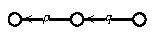
\includegraphics[scale=1.38]{figures/Fig_022_PDF082_Book070.pdf}
  % [Fig] 原书 p.70
\end{figure}
与顶点对应的平凡路径构成一组完全正交幂等元：对所有 $v,w\in Q_0$，
\[
  vw=\begin{cases}
    v,&v=w,\\
    0,&v\ne w,
  \end{cases}
  \qquad\text{并且}\qquad
  \sum_{v\in Q_0}v=1.
\]
\end{definition}

这些幂等元张成半单子代数 $\mathbb C Q_0$。所有非平凡路径张成双边理想
\[
  J=\langle a\mid a\in Q_1\rangle\subset\mathbb C Q.
\]
% [Tutor Note: 乘积顺序务必按"从右到左"：$pq$ 表示先走 $q$ 再走 $p$，所以 $a_1\cdots a_k$ 的拼接条件是 $t(a_i)=h(a_{i+1})$（头尾相接）。若按从左到右理解，后面 $P_v(w)=v\mathbb C Qw$、$\mathbb C Q(v,w)=w\mathbb C Qv$ 和 $vw=\delta_{vw}v$ 的下标会整体反过来。]

\begin{example}[几个基本箭图及其路径代数]\label{ex:basic-quiver-path-algebras}
例如，考虑下面三个箭图：
\begin{figure}[H]\centering
    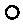
\includegraphics[scale=1.38]{figures/Fig_023_PDF083_Book071.pdf}\qquad
    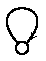
\includegraphics[scale=1.38]{figures/Fig_024_PDF083_Book071.pdf}\qquad
    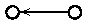
\includegraphics[scale=1.38]{figures/Fig_025_PDF083_Book071.pdf}
  % [Fig] 原书 p.71
\end{figure}
它们对应的路径代数依次为 $\mathbb C$、$\mathbb C[X]$ 和非严格上三角矩阵代数
\[
  \begin{pmatrix}\mathbb C&\mathbb C\\0&\mathbb C\end{pmatrix}.
\]
一个顶点带有 $k$ 个环箭的箭图则给出自由代数 $\mathbb C\langle X_1,\ldots,X_k\rangle$。
\end{example}

\begin{note}\phantomsection\label{note:path-algebra-as-category}
\textbf{注 4.4.} 路径代数也可以看成一个范畴 $\mathbb C Q$。其对象是顶点，两个顶点间的态射空间为
\[
  \mathbb C Q(v,w)=w\mathbb C Qv,
\]
而顶点幂等元就是恒等态射：$1_v=v\in v\mathbb C Qv$。
\end{note}

\subsection{简单模与投射模}\label{subsec:simples-projectives}
分别用 $\mathrm{mod}Q$、$\mathrm{Mod}Q$ 和 $\mathrm{MOD}Q$ 表示有限维、有限生成和所有右 $\mathbb C Q$-模构成的范畴；其 $A_\infty$ 版本分别记作 $\mathrm{mod}^\bullet Q$、$\mathrm{Mod}^\bullet Q$ 和 $\mathrm{MOD}^\bullet Q$。由 $Q_0$ 参数化的两类重要右模为：
\begin{itemize}
  \item 基本投射模\index{jibentoushemo@基本投射模|hyperpage} $P_v=v\mathbb C Q$。它也可看成反变函子
  \[
    P_v\colon\mathbb C Q\to\mathrm{VECT}(\mathbb C),\qquad
    P_v(w)=v\mathbb C Qw,
  \]
  且对箭头 $a$，有 $P_v(a)x=xa$。
  \item 基本简单模\index{jibenjiandanmo@基本简单模|hyperpage} $S_v=v\mathbb C Q/J$。它也可看成反变函子
  \[
    S_v\colon\mathbb C Q\to\mathrm{VECT}(\mathbb C),\qquad
    S_v(w)=\delta_{vw}\mathbb C,
  \]
  且 $S_v(a)=0$。
\end{itemize}

由于前一类模是投射模，它们之间没有非平凡扩张，因此
\[
  \operatorname{Ext}^i_{\mathbb C Q}(P_v,P_w)
  =\begin{cases}
    w\mathbb C Qv,&i=0,\\
    0,&i>0.
  \end{cases}
\]
这说明，导出范畴 $D\mathrm{MOD}^\bullet Q$ 中包含所有基本投射模的全子范畴 $P^\bullet$，同构于集中在次数 $0$、高阶乘积全为零的 $A_\infty$ 范畴 $\mathbb C Q$。

简单模 $S_v$ 有如下投射分解：
\[
  \bigoplus_{h(a)=v}P_{t(a)}\xrightarrow{\,a\cdot\,}P_v.
\]
由此容易算得
\[
  \operatorname{Ext}^i_{\mathbb C Q}(S_v,S_w)=
  \begin{cases}
    \delta_{vw}\mathbb C,&i=0,\\
    \mathbb C^{\oplus\#\{a:v\leftarrow w\}},&i=1,\\
    0,&i>1.
  \end{cases}
\]
% [Tutor Note: $\operatorname{Ext}^1(S_v,S_w)$ 的指标方向最容易写反：它是 $\#\{a:v\leftarrow w\}$，即从 $w$ 指向 $v$ 的箭头数。原因在投射分解 $\bigoplus_{h(a)=v}P_{t(a)}\to P_v$：同调计算给出 $\operatorname{Ext}^1(S_v,S_w)=\operatorname{Hom}(P_{t(a)},S_w)$，只在存在满足 $h(a)=v$、$t(a)=w$ 的箭头时非零。用单箭头箭图 $v_1\to v_2$ 验算：$\operatorname{Ext}^1(S_2,S_1)=\mathbb C$，而 $\operatorname{Ext}^1(S_1,S_2)=0$。]

令 $S=\bigoplus_{v\in Q_0}S_v$。则 $\operatorname{Ext}^\bullet_{\mathbb C Q}(S,S)$ 是一个分次向量空间，由每个顶点 $v\in Q_0$ 对应的次数 $0$ 元素 $v^*=1_{S_v}$ 和每个箭头 $a\in Q_1$ 对应的次数 $1$ 元素 $a^*$ 张成。次数 $0$ 与次数 $1$ 元素之间的乘积顺序反转，因此可把 $v^*$ 和 $a^*$ 看作反向箭图的顶点和箭头。两个次数 $1$ 元素的乘积为零，因为不存在次数 $2$ 的元素。于是得到如下 Ext 环：
\[
  \operatorname{Ext}^\bullet_{\mathbb C Q}(S,S)
  =\mathbb C Q^{\mathrm{op}}/\langle a^*b^*\mid a^*b^*\text{ 是长度为 }2\text{ 的路径}\rangle.
\]
仿照对偶数环（例\ref{ex:dual-numbers-ext}），我们把这个代数称为对偶箭图代数\index{duioujiantudaishu@对偶箭图代数|hyperpage}，记作 $\Lambda_Q$。由于不存在次数 $2$ 的元素，$\Lambda_Q$ 上的高阶乘积全为零。这说明，导出范畴 $D\mathrm{MOD}^\bullet Q$ 中包含所有基本简单模的全子范畴 $S^\bullet$，严格同构于高阶乘积全为零的 $A_\infty$ 范畴 $\Lambda_Q$。

\begin{theorem}{箭图导出范畴的包含关系}{quiver-derived-inclusions}
对任意箭图 $Q$，都有以下 $A_\infty$ 范畴的包含关系：
\[
  DS^\bullet\subset D\mathrm{mod}^\bullet Q\subset DP^\bullet.
\]
若 $Q$ 没有有向圈，则这些包含关系都是等价。
\end{theorem}
\begin{proof}[证明思路]
第一个包含关系显然成立，因为简单模都是一维的。第二个包含关系来自每个模 $M$ 都有如下标准投射分解：
\[
  \bigoplus_{a\in Q_1}M_{h(a)}\otimes_{\mathbb C}P_{t(a)}
  \xrightarrow{\ d\ }
  \bigoplus_{v\in Q_0}M_v\otimes_{\mathbb C}P_v.
\]
在箭头 $a$ 对应的分量上，微分由模作用与路径拼接之差给出：
\[
  d(m_a\otimes x_a)=m_a a\otimes x_a-m_a\otimes ax_a.
\]
若 $M$ 是有限维模，则分解两端都是有限个投射模的直和，因此该分解是 $P^\bullet$ 上的扭曲复形。

当 $Q$ 没有有向圈时，由于路径只有有限多条，基本投射模都是有限维的。此外，简单模只有 $S_v$，而 $\mathbb C Q$（从而所有基本投射模）都由基本简单模生成。因此 $DP^\bullet\subset DS^\bullet$。
\end{proof}

\begin{note}\phantomsection\label{note:quiver-oriented-cycles}
\textbf{注 4.6.} 若 $Q$ 有有向圈，则上述三个范畴两两不同：$DS^\bullet$ 只包含幂零模，即那些经由某个 $\mathbb C Q/J^k$ 因子化的模（$k\geq1$）；而 $D\mathrm{mod}^\bullet Q$ 不包含那些对应顶点位于有向圈上的基本投射模 $P_v$。
\end{note}

\subsection{扭曲复形}\label{subsec:quiver-twisted-complexes}
为在 $D\mathrm{mod}^\bullet Q$、$DP^\bullet$ 和 $DS^\bullet$ 之间方便地转换，我们引入箭图表示\index{jiantubiaoshi@箭图表示|hyperpage}的概念。

\begin{definition}{维数向量与箭图表示}{quiver-representation}
箭图 $Q$ 的维数向量\index{weishuxiangliang@维数向量|hyperpage}是映射 $\alpha\colon Q_0\to\mathbb N$，其大小定义为 $|\alpha|=\sum_{v\in Q_0}\alpha_v$。一个 $\alpha$ 维表示是下列空间的元素：
\[
  \rho\in\operatorname{Rep}(Q,\alpha)
  :=\prod_{a\in Q_1}\operatorname{Mat}_{\alpha_{h(a)}\times\alpha_{t(a)}}(\mathbb C).
\]
\end{definition}

表示 $\rho$ 有三种解释方式：
\begin{itemize}
  \item 它是右 $\mathbb C Q$-模 $M_\rho\colon\mathbb C Q\to\mathrm{vect}(\mathbb C)$：对象 $v$ 映到向量空间 $M_\rho(v):=\mathbb C^{\alpha_v}$，箭头 $a\in Q_1$ 映到线性映射
  \[
    M_\rho(a)\colon\mathbb C^{\alpha_{t(a)}}\to\mathbb C^{\alpha_{h(a)}},
    \qquad x\longmapsto\rho(a)x,
  \]
  其中 $x$ 视为列向量。
  \item 它是 $P^\bullet$ 上的扭曲复形，来自 $M_\rho$ 的标准投射分解：
  \[
    P_\rho=\left(
    \bigoplus_{a\in Q_1}P_{t(a)}^{\oplus\alpha_{h(a)}}
    \xrightarrow{\,\rho(a)-a\,}
    \bigoplus_{v\in Q_0}P_v^{\oplus\alpha_v}
    \right).
  \]
  \item 它是 $S^\bullet$ 上的扭曲复形
  \[
    S_\rho:=\left(\bigoplus_{v\in Q_0}(S_v)^{\oplus\alpha_v},
    \quad \delta=\sum_{a\in Q_1}\rho(a)^\mathsf T a^*\right),
  \]
  其中 $\rho(a)^\mathsf T a^*$ 应看作从 $(S_{h(a)})^{\oplus\alpha_{h(a)}}$ 到 $(S_{t(a)})^{\oplus\alpha_{t(a)}}$ 的矩阵块。由于各个 $a^*$ 之间的乘积都为零，Maurer–Cartan 方程自动成立；但 $\delta$ 未必下三角，所以 $S_\rho$ 未必是扭曲复形。只有当 $M_\rho$ 是幂零模时才是如此。
\end{itemize}

\begin{lemma}{幂零表示对应的扭曲复形}{nilpotent-representation-twisted-complex}
若 $M_\rho$ 是幂零的，则
\[
  S_\rho\simeq M_\rho\simeq P_\rho\in DP^\bullet.
\]
\end{lemma}
\begin{proof}[证明思路]
利用顶点简单模的标准投射分解，可将 $S_\rho$ 变换为 $P_\rho$；再对 $P_\rho$ 取余核，即可得到 $M_\rho$。
\end{proof}

\begin{theorem}{简单模导出范畴的对象分类}{objects-in-derived-simples}
$DS^\bullet$ 中的每个对象都同构于若干个 $S_\rho$ 的移位的直和。
\end{theorem}
\begin{proof}[证明思路]
首先证明每个 $(M,\delta)$ 都同构于这样一个复形：其扭曲项 $\delta$ 中不含顶点恒等态射 $v^*$；对直和项的个数作归纳即可。若只有一个直和项，则 $\delta=0$，结论显然。

取一个扭曲复形 $(M,\delta)$，考察 $\delta$ 的最底行。由归纳假设，可以设 $\delta$ 的其他行只含对偶箭头。共轭变换（见第~\ref{note:conjugation-twisted-complex}~节的注）后，可保证最底行至多出现一个顶点 $v^*=1_{S_v}$。

这个顶点态射连接两个直和项 $S_v[i+1]\xrightarrow{1}S_v[i]$：
\begin{figure}[H]\centering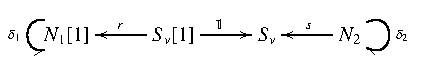
\includegraphics[width=0.72\textwidth]{figures/Fig_026_PDF086_Book074.pdf}
  % [Fig] 原书 p.74
\end{figure}
若 $(M,\delta)$ 不能分解为两个更小复形的直和，则所有其他直和项都通过含对偶箭头的分量与 $S_v[i+1]$ 或 $S_v[i]$ 相连；由于次数限制，它们不可能同时与两者相连。由 $\delta^2=0$ 可知，从 $S_v[i]$ 出发或到达 $S_v[i+1]$ 的分量均为零。于是该复形（相差一个移位）具有图示的形状，并可通过两条拟同构变换为较小复形
\[
  (M_{\mathrm{red}},\delta_{\mathrm{red}})
  =(N_1\oplus N_2[1],\delta_1+\delta_2).
\]
\begin{figure}[H]\centering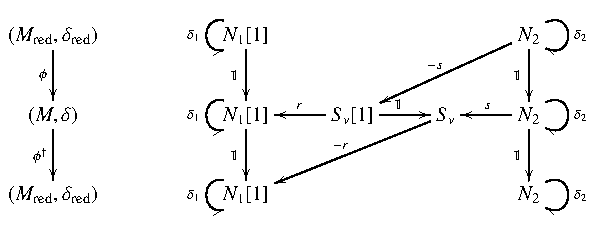
\includegraphics[width=0.94\textwidth]{figures/Fig_027_PDF086_Book074.pdf}
  % [Fig] 原书 p.74
\end{figure}

若一个扭曲复形的 $\delta$ 中只有对偶箭头，则可将其写成所有直和项具有相同移位次数的复形的直和。这样的复形形如 $S_\rho[i]$，其中 $\rho(a)$ 是 $a^*$ 系数构成的矩阵。\end{proof}

\begin{note}\phantomsection\label{note:hereditary-quiver}
\textbf{注 4.10.} 更一般地，可以证明 $D\mathrm{MOD}^\bullet Q$ 中每个对象都同构于若干个模（微分为零的复形）的移位的直和。这是表示论中的经典定理，源于 $\mathbb C Q$ 是遗传代数\index{yichuandaishu@遗传代数|hyperpage}：投射 $\mathbb C Q$-模的子模仍然是投射模。
\end{note}

\section{弦与带}\label{sec:strings-bands}
\takeaway{三种箭图的不可分解对象都有曲线模型：线性箭图 $\leftrightarrow$ $(n+1)$ 边形中的分次线段 $S_{ij}$，克罗内克箭图 $\leftrightarrow$ 圆柱上的弦对象与带对象（后者带秩 $n$ 局部系统），循环箭图 $\leftrightarrow$ 带无穷远端的圆柱上的曲线；态射是交点处的角，乘积由多边形与沿边平行传输给出。}
利用前面建立的形式体系，我们现在考察三个特殊箭图，并将其表示论解释为曲面上线段的交理论。对大多数箭图，不可能分类所有不可分解表示；只有当底层图是 Dynkin 图或扩展 Dynkin 图时，才有完整分类。下面要研究的三个箭图都属于这两类。

\subsection{线性箭图}\label{subsec:linear-quiver}
令 $Q=L_n$ 为有 $n$ 个顶点的线性箭图：
\begin{figure}[H]\centering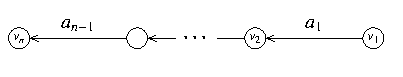
\includegraphics[scale=1.38]{figures/Fig_028_PDF087_Book075.pdf}
  % [Fig] 原书 p.75
\end{figure}
顶点从左到右记作 $v_1,\ldots,v_n$，箭头记作 $a_1,\ldots,a_{n-1}$。顶点简单模记作 $S_i$，对偶箭图中的箭头记作 $\alpha_i=a_i^*$：
\begin{figure}[H]\centering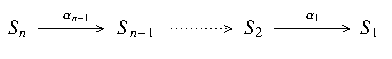
\includegraphics[scale=1.38]{figures/Fig_029_PDF087_Book075.pdf}
  % [Fig] 原书 p.75
\end{figure}

对每一对 $1\leq i\leq j\leq n$，都有一个扭曲复形
\[
  S_{ij}=\left(S_i\oplus\cdots\oplus S_j,
  \delta=\alpha_i+\cdots+\alpha_{j-1}\right).
\]
它对应如下模：顶点 $v_i,\ldots,v_j$ 映到一维向量空间，其间的箭头映到非零映射。等价地，它对应表示 $\rho_{ij}$，其维数向量为
\[
  \varepsilon_{ij}=(0,\ldots,0,1,\ldots,1,0,\ldots,0),
\]
且当 $i\leq k<j$ 时 $\rho_{ij}(a_k)=1$。

\begin{theorem}{线性箭图的不可分解对象}{linear-quiver-indecomposables}
$DS^\bullet$ 中所有不可分解对象都同构于某个 $S_{ij}$ 的移位。
\end{theorem}
\begin{proof}[证明思路]
由定理\ref{thm:objects-in-derived-simples}，$DS^\bullet$ 中每个不可分解对象都是某个 $S_\rho$ 的移位。由于每个对偶顶点恰好有一条 $\alpha_i$ 射出、也恰好有一条 $\alpha_i$ 射入，不可分解的 $S_\rho$ 必须具有如下形式：
\[
  \left(S_i^{\oplus m_i}\oplus S_{i+1}^{\oplus m_{i+1}}
  \oplus\cdots\oplus S_j^{\oplus m_j},
  \quad B_i\alpha_i+\cdots+B_{j-1}\alpha_{j-1}\right),
\]
其中 $B_k$ 是一个元素属于 $\mathbb C$ 的 $m_k\times m_{k+1}$ 矩阵。

将 $\mathbb C^{m_k}$ 分解为 $\operatorname{Im}B_k\oplus R$。若 $R\ne0$，则
\[
  \cdots\oplus B_{k-2}B_{k-1}R\otimes S_{k-2}
  \oplus B_{k-1}R\otimes S_{k-1}\oplus R\otimes S_k
\]
是一个直和项，因此 $B_k$ 必须满射。同理，$B_k$ 也必须单射，否则
\[
  \ker B_k\otimes S_{k-1}\oplus B_{k+1}^{-1}\ker B_k\otimes S_k
  \oplus B_{k+2}^{-1}B_{k+1}^{-1}\ker B_k\otimes S_{k+1}\oplus\cdots
\]
会成为一个直和项。因此所有 $B_k$ 都可逆，并且可通过共轭变换（见第~\ref{note:conjugation-twisted-complex}~节的注）将它们化为单位矩阵。若各矩阵都是 $r\times r$，该扭曲复形便分解为 $r$ 个形如 $S_{ij}$ 的子复形。\end{proof}

确定了不可分解对象之后，下一步是研究它们之间的态射。由定义可得
\[
\begin{aligned}
  \operatorname{Tw}S^\bullet(S_{ij},S_{kl})
  &=\bigoplus_{\substack{i\leq u\leq j<本地路径> u\leq l}}\mathbb C1_{S_u}
  \oplus\bigoplus_{\substack{i\leq v+1\leq j<本地路径> v\leq l}}\mathbb C\alpha_v,
\end{aligned}
\]
其中 $d\alpha_v=0$，而
\[
  d1_{S_u}=\alpha_{u-1}-\alpha_u,
\]
除非 $\alpha_{u-1}$ 或 $\alpha_u$ 不在 $\operatorname{Tw}S^\bullet(S_{ij},S_{kl})$ 中；若不在，就从求和中删去相应项。计算上同调后得到下表。

\begin{lemma}{线性箭图中扭曲复形的态射}{linear-quiver-morphism-table}
设 $S_{ij}$、$S_{kl}$ 是上述扭曲复形，则
\[
\begin{array}{c|c|c}
\text{情形}&DS^0(S_{ij},S_{kl})&DS^1(S_{ij},S_{kl})\\\hline
i-1\leq k-1<j\leq l&\mathbb C\,\iota&0\\
k-1<i-1\leq l<j&0&\mathbb C\,\gamma\\
\text{其他情形}&0&0
\end{array}
\]
次数 $0$ 元素为 $\iota=\sum_u1_{S_u}$，求和遍历两个区间的所有重叠顶点。次数 $1$ 元素为 $\gamma=\alpha_v$（任选一个这样的 $\alpha_v$ 即可；它们在上同调中彼此相等）。
\end{lemma}

这一规则可以从几何角度理解：把扭曲复形看成多边形中的线段。
\begin{definition}{多边形中的分次线段}{graded-line-segment}
取一个正则 $(n+1)$ 边形，顶点为 $p_0,\ldots,p_n$，按逆时针编号，并假设边 $p_np_0$ 是多边形底部的水平边。分次线段\index{fencixianduan@分次线段|hyperpage}是一个二元组 $L=(\overrightarrow{p_ip_j},\theta)$，其中 $\overrightarrow{p_ip_j}$ 是连接两个顶点的有向线段，$\theta\in\mathbb R$ 是相位\index{xiangwei@相位|hyperpage}，满足 $\theta$ 模 $2\pi$ 等于该线段与 $X$ 轴的夹角。

每条 $\overrightarrow{p_ip_j}$ 都可以赋予多个相位，它们相差 $2\pi$ 的整数倍。反转线段方向时，相位必须加上 $\pi$。因此记
\[
  L[k]:=(\overrightarrow{p_jp_i},\theta+k\pi).
\]
每个分次线段都是下列某条线段的移位：
\[
  L_{ij}:=(\overrightarrow{p_{i-1}p_j},\theta),
  \qquad \theta\in(0,2\pi].
\]
\end{definition}

\begin{figure}[H]\centering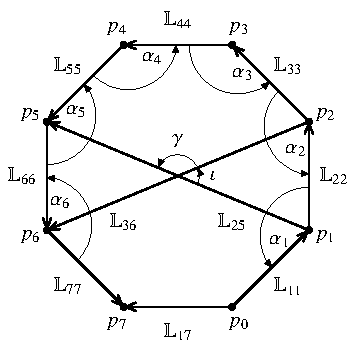
\includegraphics[width=0.95\textwidth]{figures/Fig_030_PDF089_Book077.pdf}
  % [Fig] 原书 p.77
\end{figure}
若把分次线段 $L_{ij}[k]$ 解释为表示 $S_{ij}[k]$，就会看到基本简单模 $S_i=S_{ii}$ 对应多边形的各条边，只有水平底边例外；在图示的八边形情形中，该边对应 $S_{17}$（注意它的定向相反）。两个简单模之间存在次数 $1$ 的态射（扩张），当且仅当对应线段相接。从这一角度看，相应的态射 $\alpha_i$ 就是多边形的角。

这一解释也适用于其他表示。$S_{25}$ 与 $S_{36}$ 之间有两个态射：次数 $0$ 态射 $\iota\colon S_{25}\to S_{36}$；另有次数 $1$ 态射 $\gamma\colon S_{36}\to S_{25}$。从图中可见，线段 $L_{25}$ 和 $L_{36}$ 在多边形内部相交，交点处有两个角，分别朝向两个方向。

\begin{proposition}{观察：态射是角}{morphisms-are-angles}
设 $L_1,L_2$ 是分别对应于分次线段 $(\ell_1,\theta_1)$ 和 $(\ell_2,\theta_2)$ 的两个扭曲复形。若底层线段不同，则
\[
  DS^\bullet(L_1,L_2)\ne0
\]
当且仅当多边形内部存在一个从 $L_1$ 指向 $L_2$ 的正角 $\beta\in[0,\pi)$。此时态射空间由一个次数为
\[
  \frac{\beta-(\theta_2-\theta_1)}{\pi}
\]
的态射生成。该次数衡量转角与相位变化之差。
% [Tutor Note: 次数公式 $\deg=\bigl(\beta-(\theta_2-\theta_1)\bigr)/\pi$ 中 $\beta$ 与 $\theta_i$ 都以逆时针为正；把某个相位换成等价的 $\theta+2\pi$ 不改变次数，但把线段的定向改取相反代表元会同时给 $\beta$ 与 $\theta$ 加 $\pi$，次数保持不变。实践中最容易出错的是只给其中一个量加 $\pi$，结果整体差一次移位。]
\end{proposition}

这种解释也有助于构造锥。再看上图，可以发现：
\begin{itemize}
  \item $\alpha_i\colon S_{i+1}\to S_i$ 的锥为 $S_{i,i+1}$，几何上可看成用角 $\alpha_i$ 将 $S_i$ 和 $S_{i+1}$ 对应的线段拼接，再将拐角拉直。
  \item $\gamma\colon S_{36}\to S_{25}$ 的锥为
  \[
    \left(S_2\oplus S_3\oplus S_4\oplus S_5
    \oplus S_3\oplus S_4\oplus S_5\oplus S_6,
    \alpha_3+\alpha_4+\alpha_5+\alpha_4+\alpha_5+\alpha_6+\gamma\right).
  \]
  重新排列后，它同构于 $S_{26}\oplus S_{35}$。从几何上看，我们使用角 $\gamma$ 以另一种方式拼接线段。
  \item 把次数 $1$ 态射 $\iota\colon S_{25}\to S_{36}$ 看成 $\iota\colon S_{25}[1]\to S_{36}$，取其锥可得
  \[
    \left(S_2[1]\oplus\cdots\oplus S_5[1]\oplus S_3\oplus\cdots\oplus S_6,
    -\alpha_3-\alpha_4-\alpha_5+\alpha_4+\alpha_5+\alpha_6
    +1_{S_3}+1_{S_4}+1_{S_5}\right),
  \]
  由定理\ref{thm:objects-in-derived-simples}的证明方法可知，它同构于 $S_2[1]\oplus S_6$。这里同样是利用角把线段拼接起来。
\end{itemize}

\begin{proposition}{观察：锥是拼接}{cones-are-stitches}
设 $L_1,L_2$ 是相位属于 $(0,2\pi)$ 的两条分次线段，$\alpha$ 是对应于次数 $1$ 态射的角。取 $\alpha$ 的锥，在几何上就是沿着 $\alpha$ 将两条线段拼接所得的线段。
\end{proposition}
\begin{figure}[H]\centering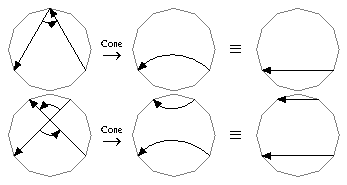
\includegraphics[width=0.78\textwidth]{figures/Fig_031_PDF090_Book078.pdf}
  % [Fig] 原书 p.78
\end{figure}

几何解释的最后一部分涉及乘积。位于多边形同一顶点的边界角相乘时，会合成为一个角；那么内部角又如何相乘？我们再看两个例子。
\begin{itemize}
  \item 取扭曲复形 $A=S_{36}$、$B=S_{25}$、$X=S_{47}$、$Y=S_{35}$。有次数 $0$ 态射 $\iota_{AX}\colon S_{36}\to S_{47}$ 和次数 $1$ 态射 $\gamma_{XB}\colon S_{47}\to S_{25}$。它们的复合是次数 $1$ 态射 $\gamma_{AB}\colon S_{36}\to S_{25}$。从图中可见，$\iota_{AX}$ 和 $\gamma_{XB}$ 是一个三角形的内部角，而 $\gamma_{AB}$ 是第三个顶点处的外角。
  \item $\iota_{BY}\colon S_{25}\to S_{35}$ 与 $\iota_{YA}\colon S_{35}\to S_{36}$ 的乘积是 $\iota_{BA}\colon S_{25}\to S_{36}$；后者是以 $\iota_{BY}$ 和 $\iota_{YA}$ 为内角的三角形在第三个顶点处的外角。
\end{itemize}
\begin{figure}[H]\centering
  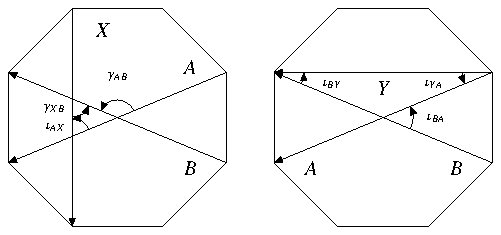
\includegraphics[width=0.44\textwidth]{figures/Fig_032_PDF091_Book079.pdf}\hfill
  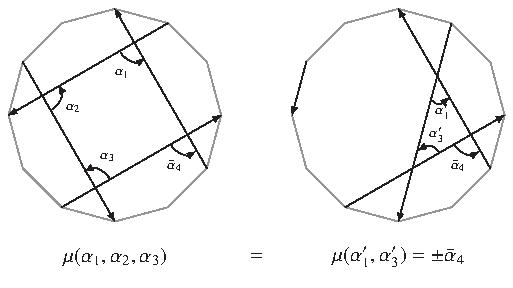
\includegraphics[width=0.44\textwidth]{figures/Fig_033_PDF091_Book079.pdf}
  % [Fig] 原书 p.79
\end{figure}

因此，乘积对应三角形。这一观察甚至可推广到高阶乘积。若有一个内部 $n$ 边形，想要对其中 $n-1$ 个内部角取高阶乘积，就可以对其中一个态射取锥，把问题改写为 $(n-2)$ 元乘积（见引理\ref{lem:higher-products-and-cones}）。取锥会把两条边拼在一起，形成一个 $(n-2)$ 边形。重复这一过程，最后得到一个三角形，便可用二元乘积规则解释：
\[
  \mu(\alpha_1,\alpha_2,\alpha_3)
  =\mu(\alpha'_1,\alpha'_3)=\pm\overline\alpha_4.
\]
\begin{figure}[H]\centering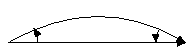
\includegraphics[width=0.72\textwidth]{figures/Fig_034_PDF092_Book080.pdf}
  % [Fig] 原书 p.80
\end{figure}

\begin{proposition}{观察：多边形诱导乘积}{polygons-induce-products}
若 $L_1,\ldots,L_k$ 是围成一个子多边形的线段，则除一个角以外，所有连接这些线段的内部态射的高阶乘积，等于剩余顶点处的外角态射：
\[
  \mu(\alpha_1,\ldots,\alpha_{k-1})=\pm\overline\alpha_k.
\]
符号取决于这些态射的次数。
\end{proposition}

\begin{note}\phantomsection\label{note:degenerate-polygons}
\textbf{注 4.17.} 请注意，$DS^\bullet$ 中并非每个非零乘积都来自一个多边形，因为有时对应的多边形会退化（例如三条线段经过同一点，或其中若干线段重合）。
\end{note}

\begin{proposition}{观察：线段交理论}{intersection-theory-line-segments}
$A_\infty$ 范畴 $DS^\bullet$ 描述了多边形中线段的交理论。
\end{proposition}

\begin{note}\phantomsection\label{note:rigorous-polygon-model}
\textbf{注 4.19.} 要使这一观察严格化并不容易。一种办法是使用预范畴，定义如下：
\begin{itemize}
  \item 横截序列是所有两两交点彼此不同的分次线段序列；
  \item Hom 空间是由交点处各个角张成的分次 $\mathbb C$-向量空间；
  \item 唯一可能非零的乘积由观察\ref{pro:polygons-induce-products}中的规则给出。
\end{itemize}
遗憾的是，这个预范畴没有同构。为解决这一问题，可以加入分次曲线\index{fenciquxian@分次曲线|hyperpage}。分次曲线是一个二元组
\[
  L=\bigl(\gamma\colon[0,1]\to\mathbb R^2,
  \theta\colon[0,1]\to\mathbb R\bigr),
\]
其中 $\gamma$ 是多边形内连接两个不同顶点的光滑嵌入，而 $\theta(x)$ 是 $\gamma$ 在 $x$ 处的切向量与 $X$ 轴的夹角。

在这个预范畴中，图示的角都是拟同构：
\begin{figure}[H]\centering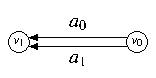
\includegraphics[width=0.52\textwidth]{figures/Fig_035_PDF093_Book081.pdf}
  % [Fig] 原书 p.81
\end{figure}
因此相应的极小模型 $\mathrm{Polygon}_{n+1}^\bullet$ 是一个具有足够多同构的预范畴。将其范畴化后，得到等价
\[
  DS^\bullet\cong_\infty\mathrm{Polygon}_{n+1}^\bullet.
\]
\end{note}

\subsection{克罗内克箭图}\label{subsec:kronecker-quiver}
接下来考察克罗内克箭图 $Q=K$。它由两个顶点 $v_0,v_1$ 和两条方向相同的箭头 $a_0,a_1$ 组成：
\begin{figure}[H]\centering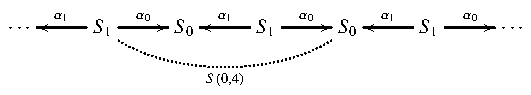
\includegraphics[width=0.28\textwidth]{figures/Fig_036_PDF093_Book081.pdf}
  % [Fig] 原书 p.81
\end{figure}

范畴 $P^\bullet$ 包含两个投射模 $P_i=v_i\mathbb C Q$，范畴 $S^\bullet$ 包含两个简单模 $S_i=v_i\mathbb C Q/\langle a_0,a_1\rangle$。这两个简单模的 Ext 环是 $\Lambda_Q$。由于不存在长度为 $2$ 的路径，$\mathbb C Q^{\mathrm{op}}\cong\mathbb C Q$。因此，范畴 $S^\bullet$ 和 $P^\bullet$ 看起来相同，但分次不同：$P^\bullet$ 中所有态射的次数都是 $0$，而 $S^\bullet$ 中对偶箭头 $\alpha_i=a_i^*$ 的次数为 $1$。

\begin{theorem}{克罗内克箭图的不可分解对象}{kronecker-quiver-indecomposables}
$DS^\bullet$ 中每个不可分解对象都同构于下列复形之一的移位：
\begin{enumerate}[label=(\roman*)]
  \item $S(i,w)$ 是下方无穷串中的一个线性子复形，它从右侧的 $S_i$ 开始，共含 $w$ 项；
  \begin{figure}[H]\centering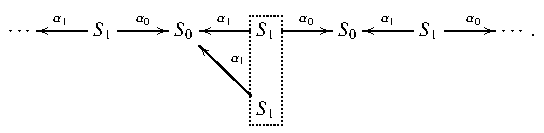
\includegraphics[width=0.91\textwidth]{figures/Fig_037_PDF094_Book082.pdf}
  % [Fig] 原书 p.82
\end{figure}
  \item
  \[
    B(\lambda,n)=\left(S_0^{\oplus n}
    \xleftarrow{\,\alpha_0 1_n+\alpha_1J(\lambda,n)\,}
    S_1^{\oplus n}\right),
  \]
  其中 $J(\lambda,n)$ 是大小为 $n$、特征值为 $\lambda\in\mathbb C^*$ 的 Jordan 块。
\end{enumerate}
\end{theorem}
\begin{proof}[证明思路]
设 $(M,\delta)$ 是一个不可分解扭曲复形。由定理\ref{thm:objects-in-derived-simples}，可设它具有如下形式：
\[
  \left(S_0[k]^{\oplus n}\oplus S_1[k]^{\oplus m},
  \quad B_0\alpha_0+B_1\alpha_1\right),
\]
其中 $B_0,B_1$ 是 $m\times n$ 矩阵。相差一个同构，我们可以分别在左、右乘同一个可逆矩阵。若 $B_0,B_1$ 都可逆，则可先把 $B_0$ 化为单位矩阵，再将 $B_1$ 共轭化为 Jordan 块，从而得到 $B(\lambda,n)$。

若 $B_0$ 或 $B_1$ 不可逆，则对 $n+m$ 作归纳，证明 $(M,\delta)$ 同构于某个 $S(i,w)$。当 $n+m=1$ 时，$(M,\delta)$ 显然是 $S_0=S(0,1)$ 或 $S_1=S(1,1)$。当 $n+m\geq2$ 时，根据 $B_i$ 是否单射、是否满射分为四种情形；这里只详述其中一种。

假设 $B_0$ 有核。取核中的一个基向量 $v$，并令 $w=B_1v$。由于扭曲复形不可分解，$w\ne0$。将 $v,w$ 分别扩充为 $\mathbb C^n$ 与 $\mathbb C^m$ 的基，可以把两个矩阵写成如下形式：
\[
  B_0=\begin{pmatrix}0&*\\0&B'_0\end{pmatrix},
  \qquad B_1=\begin{pmatrix}1&*\\0&B'_1\end{pmatrix}.
\]
通过右乘可逆矩阵，可以假定 $B_1$ 的第一行以零开头。由于 $B'_1$ 不可逆，$(B'_0,B'_1)$ 满足归纳假设，因而对应某个弦对象\index{xianduixiang@弦对象|hyperpage} $S(i,w)$。原复形于是具有原书图示的串形结构。

若最底下的 $S_1$ 在链的中部与其他项相连，则考察 $B_0,B_1$ 在虚线所示 $S_1\oplus S_1$ 上限制所得的核 $K_0,K_1$。若二者相同，则有一个同构于 $S_1$ 的直和项；若它们张成 $K_0\oplus K_1=S_1\oplus S_1$，则整个复形可拆成两个复形的直和：
\begin{figure}[H]\centering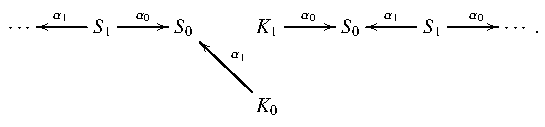
\includegraphics[width=0.91\textwidth]{figures/Fig_038_PDF094_Book082.pdf}
  % [Fig] 原书 p.82
\end{figure}
因此，在不可分解情形下，该 $S_1$ 必须连到链的一端，故整个对象就是一条链。\end{proof}

\begin{definition}{弦对象与带对象}{string-and-band-objects}
我们称 $S(i,w)$ 为弦对象，称 $B(\lambda,n)$ 为带对象\index{daiduixiang@带对象|hyperpage}。
\end{definition}

\begin{note}\phantomsection\label{note:strings-as-band-limits}
\textbf{注 4.22.} 长度为偶数的弦对象可视为带对象的极限：
\[
  \lim_{\lambda\to0}B(\lambda,n)\cong S(0,2n),
  \qquad
  \lim_{\lambda\to\infty}B(\lambda,n)\cong S(1,2n).
\]
第一个极限可直接从复形图中看出。对于第二个极限，注意到经过基变换，可以把映射 $\alpha_0 1_n+\alpha_1J(\lambda,n)$ 化为 $\alpha_0J(\lambda^{-1},n)+\alpha_1 1_n$。因此，我们有时也把这些弦对象记作 $B(0,n)$ 和 $B(\infty,n)$。
% [Tutor Note: 何以"偶长弦对象是带对象的极限"：$\lambda\to0$ 时 $J(\lambda,n)\to J(0,n)$ 成为幂零块，$\alpha_01_n+\alpha_1J(0,n)$ 的秩使复形退化为 $2n$ 项的一维链；$\lambda\to\infty$ 时首项与末项互换，得到方向相反的 $S(1,2n)$。因此带对象在参数边界上退化为偶长弦对象；对 $\lambda\in\mathbb C^*$，带对象与弦对象是不同的不可分解对象。]
\end{note}

现在为克罗内克箭图构造类似于线性箭图情形的几何解释。取一个正方形，把左右两边粘合，便得到一个圆柱；正方形的两个角分别给出圆柱两条边界圆上的标记点。圆柱是平坦曲面，可以通过提升到正方形按通常方式测量角度。与多边形情形一样，也可以定义标记点之间的分次线段。

令 $S_0$ 表示对应于正方形竖边、相位为 $\frac\pi2$ 的分次线段；令 $S_1$ 表示相位为 $\frac{5\pi}4$、方向向下的对角线。由 $S_1$ 指向 $S_0$ 有两个角，它们分别对应 $S_1$ 与 $S_0$ 之间的两个次数 $1$ 态射：
\begin{figure}[H]\centering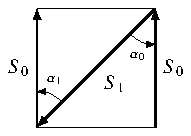
\includegraphics[width=0.56\textwidth]{figures/Fig_039_PDF095_Book083.pdf}
  % [Fig] 原书 p.83
\end{figure}

在线性箭图的多边形模型中，我们已把取锥解释为沿一个角拼接线段。同样，每个弦对象 $S(i,w)$ 都可看成圆柱普遍覆盖空间中的一条线段：
\begin{figure}[H]\centering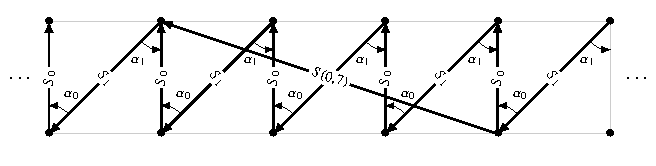
\includegraphics[width=0.96\textwidth]{figures/Fig_040_PDF095_Book083.pdf}
  % [Fig] 原书 p.83
\end{figure}

带对象又如何解释？还有另一类相位恒定的曲线：绕圆柱一周的圆。若要用这些圆解释带对象，还需附加几何数据，即局部系统\index{jubuxitong@局部系统|hyperpage}。

\begin{definition}{局部系统}{local-system}
流形 $M$ 上的局部系统是其基本群胚的一个表示
\[
  L\colon\Pi_1(M)\to\mathrm{vect}(\mathbb C).
\]
局部系统 $L$ 给每个点 $p$ 配一个向量空间 $L(p)$，称为 $p$ 上的纤维；对任意两个点之间每条路径的同伦类，还给出这些向量空间之间的一个可逆映射，有时称为沿该路径的平行传输。若 $M$ 连通，则所有纤维维数相同，称为局部系统的秩\index{zhi@秩|hyperpage}。
\end{definition}

\begin{lemma}{圆上的不可分解局部系统}{indecomposable-local-systems-circle}
圆周 $S^1$ 上的不可分解局部系统由可逆 Jordan 块分类。
\end{lemma}
\begin{proof}[证明思路]
圆周的基本群胚等价于群 $\mathbb Z$。因此，同构意义下，一个表示 $\varphi\colon\mathbb Z\to\mathrm{GL}_n$ 由可逆矩阵 $\varphi(1)$ 的共轭类确定，而该矩阵可化为 Jordan 标准形。
\end{proof}

在圆柱中固定一条水平圆，则每个带对象 $B(n,\lambda)$ 都可与这条圆上的一个局部系统对应；沿圆周的平行传输由大小为 $n$、特征值为 $\lambda$ 的 Jordan 块给出。我们把嵌入的圆及其局部系统一并记作 $B(n,\lambda)$。

弦对象也可以看成带有秩 $1$ 局部系统的线段。可缩空间上的局部系统由其秩分类，而秩为 $n$ 的局部系统是 $n$ 个秩 $1$ 局部系统的直和。因此，$S_0\oplus S_0$ 既可以看成两条各带秩 $1$ 局部系统的线段，也可以看成一条带秩 $2$ 局部系统的线段。今后默认每条分次线段 $L$ 都带有一个局部系统，并用 $L(p)$ 表示 $p$ 处的纤维。

为处理这些局部系统，还需升级态射空间。交点 $p$ 周围的每个角都应看成两个局部系统在 $p$ 处纤维之间的一个态射。因此，若 $L_1,L_2$ 是分别位于两条不同线段上的局部系统，则令
\[
  \operatorname{Hom}(L_1,L_2)
  =\bigoplus_{\alpha_p}\mathrm{vect}(L_1(p),L_2(p))_{\alpha_p},
\]
其中 $\alpha_p$ 表示交点 $p$ 处的一个角。换言之，每个角都带有一个线性映射作为系数。

这一想法与取锥构造相容。若要用态射 $f\alpha_p$ 将两个局部系统拼接起来，其中 $f\colon L_1(p)\to L_2(p)$ 可逆，就用 $f$ 识别两处纤维。若 $f$ 不可逆，则将局部系统分解为 $f$ 可逆的部分和 $f$ 为零的部分，只拼接前一部分。

带对象 $B(n,\lambda)$ 可看成分别位于 $S_0$ 和 $S_1$ 上的两个秩为 $n$ 的局部系统：一端用恒等映射拼接，另一端用 Jordan 块拼接。合起来得到一条与圆同伦的曲线，其局部系统的平行传输恰好等于该 Jordan 块；这就是 $B(n,\lambda)$。

最后还需调整乘积规则。乘积中的角系数必须双线性地纳入乘积，但连续相乘的角并不连接同一个交点处的纤维，所以这些线性映射无法直接相乘。局部系统可以解决这一问题。若多边形的一条边 $e\colon p\to q$ 位于 $L_i$ 上，则局部系统给出纤维间的映射
\[
  L_i(e)\colon L(p)\to L(q).
\]
于是可以把这些映射串接起来，定义扩展乘积：
\[
\begin{aligned}
  \mu(f_1\alpha_1,\ldots,f_4\alpha_4)
  ={}&L_1(e_0)f_1L_1(e_1)\cdots L_1(e_3)f_4L_k(e_4)\cdot\overline\alpha_0\\
    &+\cdots.
\end{aligned}
\]
\begin{figure}[H]\centering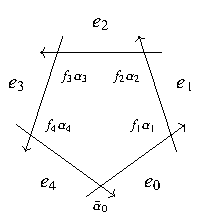
\includegraphics[width=0.58\textwidth]{figures/Fig_041_PDF097_Book085.pdf}
  % [Fig] 原书 p.85
\end{figure}
若这些角围成不止一个多边形，就把相应表达式求和。加入这些结构后，可以验证，线性箭图情形中对 $DS^\bullet$ 的观察同样适用于克罗内克箭图。

\begin{proposition}{观察：局部系统与多边形乘积}{local-systems-and-polygon-products}
$DS^\bullet$ 中的对象可识别为带有局部系统的分次线段的直和。态射是由局部系统纤维间映射加权的角；多边形对乘积的贡献，则由沿边界的总平行传输加权。
\end{proposition}

\subsection{循环箭图}\label{subsec:cyclic-quiver}
最后考察循环箭图 $Q=C_n$。它有 $n$ 个顶点 $v_1,\ldots,v_n$ 和 $n$ 条箭头 $a_i\colon v_i\to v_{i+1}$，下标按模 $n$ 计算：
\begin{figure}[H]\centering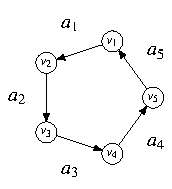
\includegraphics[width=0.48\textwidth]{figures/Fig_042_PDF097_Book085.pdf}
  % [Fig] 原书 p.85
\end{figure}

我们允许 $n=1$，此时箭图只有一个顶点和一个环箭。范畴 $P^\bullet$ 中有 $n$ 个投射模 $P_i=v_i\mathbb C Q$，范畴 $S^\bullet$ 中有 $n$ 个简单模 $S_i=v_i\mathbb C Q/J$。对偶箭头 $\alpha_i=a_i^*$ 是从 $S_{i+1}$ 到 $S_i$ 的次数 $1$ 态射。

情形与前两个例子略有不同：由于存在任意长度的路径，$\mathbb C Q$ 是无限维的。取所有长度为 $n$ 的路径之和，可得 $\mathbb C Q$ 中的一个中心元素，记作
\[
  \ell=a_n\cdots a_1+a_1a_n\cdots a_2+\cdots
  +a_{n-1}\cdots a_1a_n.
\]
容易验证，$\mathbb C[\ell]$ 是多项式环，而 $\mathbb C Q$ 是一个自由 $\mathbb C[\ell]$-模，其基由所有长度小于 $n$ 的路径组成。由于 $\mathbb C Q$ 是无限维的，三个范畴
\[
  DS^\bullet\subset D\mathrm{mod}^\bullet Q\subset DP^\bullet
\]
彼此不同；分类定理也体现了这一点。

\begin{theorem}{循环箭图投射导出范畴中的不可分解对象}{cyclic-quiver-projective-indecomposables}
$DP^\bullet$ 中的不可分解对象都是下列对象之一的移位：
\begin{itemize}
  \item
  \[
    S(i,w)=\left(S_i\oplus\cdots\oplus S_{i+w-1},
    \alpha_i+\cdots+\alpha_{i+w-1}\right);
  \]
  \item $B(k,\lambda)=M_\rho$，其中 $\rho(a_n)=J(k,\lambda)$，且对 $i\ne n$ 有 $\rho(a_i)=1_k$；
  \item $P_i$。
\end{itemize}
这里 $i\in\{1,\ldots,n\}$、$\lambda\in\mathbb C$、$w\in\mathbb N$。并且
\[
  S(i,w)\in DS^\bullet,\qquad
  B(k,\lambda)\in D\mathrm{mod}^\bullet Q,\qquad
  P_i\in DP^\bullet.
\]
\end{theorem}
\begin{proof}[证明思路]
$DP^\bullet$ 中每个不可分解对象都是一个有限生成 $\mathbb C Q$-模 $M$ 的移位。若 $M$ 是无限维的，则存在单射 $P_v\to M$；由于 $P_v$ 是投射模，该单射分裂，因此 $M\cong P_v$。

若 $M$ 是有限维的，则 $M=M_\rho$。由于 $\ell$ 是中心元，可按 $\ell$ 的特征值将 $M$ 分解为直和。因此，不可分解情形下 $\ell$ 只有一个特征值 $\lambda$。若 $\lambda\ne0$，则所有 $\rho(a_i)$ 都可逆；通过共轭，可将除 $\rho(a_n)$ 之外的矩阵化为单位矩阵，而 $\rho(a_n)$ 可化为 Jordan 块。若 $\lambda=0$，则该模是幂零模，因而属于 $DS^\bullet$。最后仿照定理\ref{thm:kronecker-quiver-indecomposables}的论证即可完成分类。
\end{proof}

这一分类同样可以解释为曲面上的曲线。取一个圆盘，中心有一个标记点，边界上有 $n$ 个标记点。把 $n$ 个简单对象对应到边界上逆时针排列的 $n$ 条弧，把 $n$ 个投射对象对应到由中心向外辐射的线段。对象 $B(k,\lambda)$ 则对应绕中心一周、并带有平行传输为 $J(k,\lambda)$ 的局部系统的曲线：
\begin{figure}[H]\centering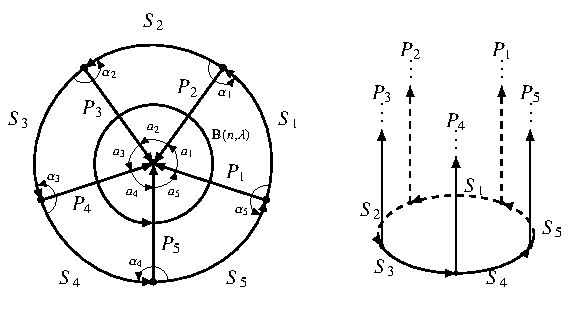
\includegraphics[width=0.92\textwidth]{figures/Fig_043_PDF099_Book087.pdf}
  % [Fig] 原书 p.87
\end{figure}

箭图的箭头对应投射模之间的态射，可看成中心标记点周围的角；对偶箭头在简单模之间给出态射，可看成圆周标记点附近的角。

乍看之下，一切都吻合，除了分次：若在欧氏平面中测量角度，则从 $P_1$ 到自身的态射 $a_n\cdots a_1$ 绕转 $2\pi$，因而必须有次数 $2$。解决办法是把曲面看成带有一个无穷远端的圆柱，而不是圆盘。此时各线段 $P_i$ 的相位为 $\frac\pi2$，而 $S_i$ 的相位为 $0$。由 $S_i,P_i,P_{i+1}$ 围成的三角形有两个 $\frac\pi2$ 的角和一个位于无穷远处的零角。

\begin{proposition}{观察：循环箭图的曲线模型}{cyclic-quiver-curves}
循环箭图的表示论可用带有一个无穷远端的圆柱上的曲线来解释。范畴 $DS^\bullet$ 包含位于边界圆上的线段，$D\mathrm{mod}^\bullet Q$ 包含紧致线段（即不延伸到无穷远处的线段），而 $DP^\bullet$ 还包含非紧致线段。
\end{proposition}

\section{点与层}\label{sec:points-sheaves}
\takeaway{同一批箭图也可解释为代数几何对象：单环箭图 $\leftrightarrow$ $\mathbb A^1$ 上的相干层，循环箭图 $\leftrightarrow$ 轨形 $[\mathbb A^1/\mathbb Z_n]$ 上的相干层（叉积代数 $\mathbb C[X]\star G$ 的模），克罗内克箭图 $\leftrightarrow$ $\mathbb P^1$ 上相干层（用两片 $\mathbb A^1$ 加粘合数据描述），线性箭图 $\leftrightarrow$ Landau--Ginzburg 模型的奇点范畴。}
本节将从另一种几何视角，即代数几何，回顾前三种箭图，并按与前面相反的顺序逐一讨论。

\subsection{循环箭图}\label{subsec:cyclic-quiver-sheaves}
先从只有一个环箭的箭图开始。它的路径代数是多项式环 $R=\mathbb C[X]$。这个环可以看成仿射直线 $\mathbb A^1=\mathbb C$ 上的多项式函数环。对每个点 $p\in\mathbb C$，有一个映射
\[
  \rho_p\colon R\to\mathbb C,\qquad f(X)\longmapsto f(p),
\]
它把每个函数取值于点 $p$。其核为
\[
  \mathfrak p=\{f\in R\mid f(p)=0\}=(X-p),
\]
模去这个核便得到简单模 $S_p=J(p,1)$。所有简单模都可如此得到，因此
\[
  \{\mathbb A^1\text{ 上的点}\}
  \longleftrightarrow\{R\text{ 的极大理想}\}
  \longleftrightarrow\{R\text{ 的简单模}\}.
\]

高阶 Jordan 块也有类似解释：$\rho_p$ 把每个函数映到它在 $p$ 处的函数值，而映射
\[
  R\to J(p,n)=\mathbb C[X]/(X-p)^n
\]
则把每个 $f$ 映到它在 $p$ 处的 $n$ 阶 Taylor 近似。因此，$J(p,n)$ 探测了点 $p$ 的无穷小邻域。

若 $M/\mathfrak pM\ne0$，则称模 $M$ 的支撑包含点 $p\in\mathbb A^1$。显然，$S_p$ 只支撑在 $p$，不支撑在其他点 $q$；$J(p,n)$ 也一样。但若把 $R$ 看成它自身上的模，情形就不同了：它在每个 $p$ 处都有支撑。每一点上的商空间 $R/\mathfrak p$ 都是一维向量空间，把这些空间合在一起，便得到 $\mathbb A^1$ 上的一个一维向量丛（或线丛\index{xiancong@线丛|hyperpage}）。$R$ 中每个元素 $m$ 在每个点 $p$ 上都给出 $R/\mathfrak p$ 中的一个元素，因此可看作该向量丛的截面。这个线丛是平凡的，因为元素 $1\in R$ 给出一个截面，并在每个纤维中构成一组基。由于 $\mathbb A^1$ 可缩，其上的每个向量丛都是平凡的；秩为 $n$ 的向量丛对应于投射（事实上自由）模 $R^{\oplus n}$：
\[
  \{\mathbb A^1\text{ 上的向量丛}\}
  \longleftrightarrow\{\text{投射 }R\text{-模}\}.
\]

既非投射模也非简单模的模有更精细的几何解释，称为相干层。第七章将更详细地讨论这一概念；目前只需知道，$\mathbb A^1$ 上的相干层等同于有限生成 $\mathbb C[X]$-模：
\[
  D\mathrm{Coh}^\bullet\mathbb A^1
  =D\mathrm{Mod}^\bullet\mathbb C[X].
\]

\begin{proposition}{观察：单环箭图与仿射直线上的层}{one-loop-quiver-sheaves}
单环箭图的表示可解释为仿射直线 $\mathbb A^1$ 上的层。在这一对应下，简单模 $S_p$ 变为支撑在点 $p$ 上的零维层，称为点层\index{dianceng@点层|hyperpage}；自由模 $\mathbb C[X]$ 变为平凡线丛 $\mathcal O$，也称结构层\index{jiegouceng@结构层|hyperpage}。
\end{proposition}

现在把这一几何解释推广到更高阶循环箭图。仍取仿射直线 $\mathbb A^1$，令循环群
\[
  G=\langle g\mid g^n=1\rangle\cong\mathbb Z_n
\]
左作用于其上：
\[
  g^k\cdot x=\zeta^kx,
  \qquad \zeta=e^{2\pi i/n}.
\]
除原点轨道只含一个点外，其余轨道都含 $n$ 个点。该作用诱导坐标环 $\mathbb C[X]$ 上的右作用，定义为
\[
  f\cdot g(x)=f(g\cdot x).
\]
若要取商，$\mathbb A^1/G$ 的坐标环应看作 $G$-不变函数环 $\mathbb C[X]^G$，因为不变函数在每个轨道上取值相同。这个环是 $\mathbb C[X^n]$，与 $\mathbb C[X]$ 同构，所以从这一角度看，$\mathbb A^1/G$ 似乎与 $\mathbb A^1$ 相同。

然而，这并未充分反映几何，因为 $\mathbb A^1/G$ 有一个特殊点（原点），而 $\mathbb A^1$ 上所有点看起来都相同。因此，更合适的做法是把商看成更精细的对象——轨形 $[\mathbb A^1/G]$，而不是仿射簇。

为此，引入 $G$-等变层：它是 $\mathbb A^1$ 上的一个层，并带有一个与 $G$ 在 $\mathbb A^1$ 上的作用相容的 $G$-作用。更精确地说，它是一个带 $G$-作用的 $\mathbb C[X]$-模 $M$，满足
\[
  (mf(x))\cdot g=(m\cdot g)(f(x)\cdot g).
\]
这两个作用可以合并到一个代数中：
\[
  \mathbb C[X]\star G
  :=\mathbb C\langle X,g\rangle
  /\langle gXg^{-1}-\zeta X,\ g^n-1\rangle.
\]
于是 $M$ 自然成为一个 $\mathbb C[X]\star G$-模。因此，定义 $G$-等变相干层的导出范畴
\[
  D\mathrm{Coh}^\bullet[\mathbb A^1/\mathbb Z_n]
  :=D\mathrm{Mod}^\bullet(\mathbb C[X]\star G).
\]
% [Tutor Note: 关系 $gXg^{-1}=\zeta X$ 说明 $g$ 并不固定 $X$，而是把 $X$ 的本征值旋转 $\zeta$；因此 $\mathbb C[X]\star G$ 比不变环 $\mathbb C[X]^G=\mathbb C[X^n]$ 大得多，前者的模保留了 $G$ 在纤维上的作用，这正是"轨形"与"商簇"的差别所在。$g^n=1$ 与 $gXg^{-1}=\zeta X$ 相容，因为 $\zeta^n=1$。]
这个范畴是轨形 $[\mathbb A^1/G]$ 上层范畴的合适替代，因此应把 $D\mathrm{Coh}^\bullet[\mathbb A^1/G]$ 视作 $[\mathbb A^1/G]$ 上相干层的导出范畴。

\begin{theorem}{循环箭图路径代数与叉积代数}{cyclic-quiver-crossed-product}
代数 $\mathbb C[X]\star G$ 同构于 $Q$ 为 $n$ 个顶点循环箭图时的路径代数 $\mathbb C Q$。
\end{theorem}
\begin{proof}[证明思路]
令 $\zeta=e^{2\pi i/n}$，并定义
\[
  e_k=\frac1n\sum_{i=1}^n\zeta^{ki}g^i.
\]
容易验证 $\sum_k e_k=1$ 且 $e_ie_j=\delta_{ij}e_i$。也就是说，这些元素构成一组正交幂等元。此外，
\[
  Xe_k=e_{k+1}X,
  \qquad
  X=\sum_i e_{i+1}Xe_i,
\]
下标均按模 $n$ 计算。现定义态射 $\varphi\colon\mathbb C Q\to\mathbb C[X]\star G$，把顶点映为 $e_k$，把箭头 $a_i$ 映为 $e_{i+1}Xe_i$。容易验证，$\varphi$ 是同构。
\end{proof}

\begin{proposition}{观察：循环箭图与轨形上的相干层}{cyclic-quiver-orbifold-sheaves}
循环箭图的表示论可以几何地解释为轨形上的相干层：
\[
  D\mathrm{Coh}^\bullet[\mathbb A^1/G]
  \cong_\infty D\mathrm{Mod}^\bullet\mathbb C C_n.
\]
\end{proposition}

\subsection{克罗内克箭图}\label{subsec:kronecker-quiver-sheaves}
为了给克罗内克箭图构造类似的解释，需要考察射影直线的代数几何。射影直线是在仿射直线 $\mathbb A^1$ 上添加一个无穷远点：$\mathbb P^1=\mathbb A^1\cup\{\infty\}$。用齐次坐标也可表示为
\[
  \mathbb P^1:=\{(x:y)\mid(x,y)\in\mathbb C^2\setminus\{(0,0)\}\},
\]
其中 $(x:y)$ 与其任意非零数倍 $(\lambda x:\lambda y)$ 视为相同。它可看成两条仿射直线
\[
  \{(x:1)\mid x\in\mathbb C\},\qquad
  \{(1:y)\mid y\in\mathbb C\}
\]
的并集，它们的交集为 $\mathbb C^*$。

这两条仿射直线的坐标环分别为 $R_X=\mathbb C[X]$ 和 $R_Y=\mathbb C[Y]$。在交叠处，$X,Y$ 都可视为函数，且满足 $Y=X^{-1}$。交叠部分的坐标环为
\[
  R_{XY}=\mathbb C[X,Y]/(XY-1).
\]
另一方面，$\mathbb C[X]$ 与 $\mathbb C[Y]$ 中唯一能延拓到整个 $\mathbb P^1$ 上的函数只有常数。空间与代数之间的对应关系可概括为原书所示的两个图：
\begin{figure}[H]\centering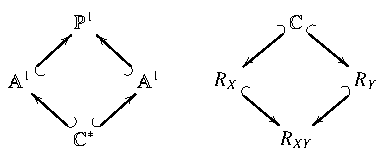
\includegraphics[width=0.78\textwidth]{figures/Fig_044_PDF102_Book090.pdf}
  % [Fig] 原书 p.90
\end{figure}

射影直线上的函数环只有 $\mathbb C$，不能充分反映其几何结构。因此，不能把 $\mathbb P^1$ 上的层看成它的坐标环上的模。解决办法是把 $\mathbb P^1$ 上的相干层视为两条仿射直线上的相干层沿交叠部分粘合而成。具体需要三项数据：有限生成 $R_X$-模 $M_X$、有限生成 $R_Y$-模 $M_Y$，以及它们在交叠处的粘合同构
\[
  \varphi_M\colon M_X\otimes_{R_X}R_{XY}
  \xrightarrow{\ \cong\ }
  M_Y\otimes_{R_Y}R_{XY}.
\]
把这个三元组 $M=(M_X,M_Y,\varphi_M)$ 称为 $\mathbb P^1$ 上的相干层。
% [Tutor Note: 粘合数据的关键在于交叠上 $Y=X^{-1}$，所以 $M_X\otimes_{R_X}R_{XY}$ 只是把 $X$ 局部化：$\mathbb C[X]/(X-\lambda)^n$ 在 $\lambda\ne0$ 时仍非零，而在 $\lambda=0$ 时归零。这正是定理 4.7（射影直线上的相干层分类）中 $S(0,n)$ 只能出现在 $X$ 片、$S(\infty,n)$ 只能出现在 $Y$ 片的原因。写 $\varphi_M$ 时勿忘它同时把 $M_X$ 一侧的 $Y$ 按 $Y=X^{-1}$ 重新解释。]

范畴 $\mathrm{Coh}\,\mathbb P^1$ 中的态射符合预期：它们是成对的模态射
\[
  (\psi_X\colon M_X\to N_X,\quad \psi_Y\colon M_Y\to N_Y),
\]
且须与粘合映射相容。可以把这些态射看作下列复形的零次同调：
\[
  \operatorname{Hom}_{R_X}(M_X,N_X)\oplus
  \operatorname{Hom}_{R_Y}(M_Y,N_Y)
  \xrightarrow{\ d^0\ }
  \operatorname{Hom}_{R_{XY}}(M_{XY},N_{XY}),
\]
其中
\[
  d^0(\psi_X\oplus\psi_Y)
  =\psi_X\otimes_{R_X}R_{XY}
  -\varphi_N^{-1}\circ(\psi_Y\otimes_{R_Y}R_{XY})\circ\varphi_M.
\]

\begin{theorem}{射影直线上的相干层分类}{coherent-sheaves-projective-line}
每个相干层都是下列几类相干层的直和：
\begin{enumerate}[label=(\roman*)]
  \item
  \[
    S(\lambda,n):=
    \left(\frac{\mathbb C[X]}{(X-\lambda)^n},
    \frac{\mathbb C[Y]}{(Y-\lambda^{-1})^n},1\right);
  \]
  \item $S(0,n):=(\mathbb C[X]/(X^n),0,0)$；
  \item $S(\infty,n):=(0,\mathbb C[Y]/(Y^n),0)$；
  \item $\mathcal O(k):=(\mathbb C[X],\mathbb C[Y],Y^k)$。
\end{enumerate}
其中 $\lambda\in\mathbb C^*$、$n\in\mathbb N$、$k\in\mathbb Z$。
\end{theorem}
\begin{proof}[证明思路]
把 $M_X$ 分解为不可分解模的直和。每个分量要么形如 $R_X/(X-\lambda)^n$（$\lambda\in\mathbb C$），要么是自由模 $R_X$。张量上 $R_{XY}$ 后，自由模仍为自由模，而
\[
  R_X/(X-\lambda)^n\quad\text{变为}\quad
  R_{XY}/(X-\lambda)^n.
\]
若 $\lambda\ne0$，后者仍是 $n$ 维的；若 $\lambda=0$，它则变为零。对 $M_Y$ 也可作同样分析，但要注意
\[
  R_{XY}/(Y-\lambda)^n\cong R_{XY}/(X-\lambda^{-1})^n.
\]

配对同构的分量可知，$M_X$ 中每个 $\mathbb C[X]/(X-\lambda)^n$ 都必须与 $M_Y$ 中一个 $\mathbb C[Y]/(Y-\lambda^{-1})^n$ 平衡，每个 $\mathbb C[X]$ 也必须与一个 $\mathbb C[Y]$ 平衡。只有 $M_X$ 中的 $\mathbb C[X]/(X^n)$ 和 $M_Y$ 中的 $\mathbb C[Y]/(Y^n)$ 不必配对，它们可拆出成为不可约相干层 $S(0,n)$ 和 $S(\infty,n)$。

其余部分需要通过同构粘合。例如，若 $M_{XY}=R_{XY}^{\oplus n}$，则粘合自同构是一个元素属于 $R_{XY}$ 的可逆 $n\times n$ 矩阵 $G$。对 $M_X=R_X^{\oplus n}$ 和 $M_Y=R_Y^{\oplus n}$ 施加自同构后，$G$ 只在右乘 $R_X$ 上的可逆矩阵、左乘 $R_Y$ 上的可逆矩阵的意义下确定。Dedekind–Weber 的经典定理说明，可以把 $G$ 化为对角矩阵，对角元是 $Y$ 的整数次幂。因此在这种情形下，该相干层是若干个 $\mathcal O(k)$ 的直和。

另一方面，形如 $R_{XY}/(X-\lambda)^n$ 的 $R_{XY}$-模之间的态射都来自 $R_X$-态射。因此可以假设这些分量之间的粘合映射就是恒等映射，得到若干个 $S(\lambda,n)$ 的直和。更多细节见\bookcite{98}、\bookcite{228}、\bookcite{109}、\bookcite{118}和\bookcite{231}。
\end{proof}

\begin{note}\phantomsection\label{note:projective-line-sheaves}
\textbf{注 4.32.} $S_\lambda:=S(\lambda,1)$ 是点层，而 $\mathcal O(k)$ 是 $\mathbb P^1$ 上的线丛。层 $\mathcal O:=\mathcal O(0)$ 是平凡线丛，也称结构层。
\end{note}

至此，我们构造了通常的相干层范畴，但还希望把它提升为一个 $A_\infty$ 范畴。正如前面用自由分解替代每个模一样，这里也可使用局部自由分解。局部自由层是三元组 $(M_X,M_Y,\varphi_M)$，其中 $M_X,M_Y$ 都是自由模。容易验证，每个相干层都有局部自由分解，可用来构造 dg-Hom 空间。

这里还有一点：如前所见，层之间的态射本身是某个复形的零次同调。因此我们实际上有两个微分；把它们相加，就得到一个大复形。$\mathrm{Coh}^\bullet\mathbb P^1$ 中的态射空间是这些复形的上同调。次数 $0$ 部分是通常的层态射，高次部分则同时度量模之间的代数扩张和粘合过程中的几何障碍。

\begin{example}[线丛之间的 dg-Hom 空间]\label{ex:dg-hom-line-bundles}
$\mathcal O(r)$ 与 $\mathcal O(s)$ 之间的 dg-Hom 空间为
\[
\underbrace{\operatorname{Hom}_{R_X}(R_X,R_X)
\oplus\operatorname{Hom}_{R_Y}(R_Y,R_Y)}_{\text{次数 }0}
\oplus
\underbrace{\operatorname{Hom}_{R_{XY}}(R_{XY},R_{XY})}_{\text{次数 }1},
\]
微分为
\[
  d(f(X)\oplus g(Y))=f(X)-X^{s-r}g(Y).
\]
若 $r>s$，第二项只含 $X$ 的负次幂，因而不可能与第一项抵消，所以零次同调为零。若 $r\leq s$，则零次同调的一组基为
\[
  (f,g)=(X^i,Y^{s-r-i}),\qquad 0\leq i\leq s-r.
\]
于是
\[
  H^0\mathrm{Coh}(\mathcal O(r),\mathcal O(s))=
  \begin{cases}
    \mathbb C(1,Y^{s-r})+\cdots+\mathbb C(X^{s-r},1),&r\leq s,\\
    0,&r>s.
  \end{cases}
\]
另一方面，一次同调是 $\mathbb C[X,X^{-1}]$ 模去由 $X^i$ 和 $X^{s-r-i}$（$i\geq0$）张成的向量空间。若 $s<r-1$，该空间非零，维数为 $r-s-1$：
\[
  H^1\mathrm{Coh}(\mathcal O(r),\mathcal O(s))=
  \begin{cases}
    0,&r\leq s+1,\\
    \mathbb CY+\cdots+\mathbb CY^{r-s-1},&r>s+1.
  \end{cases}
\]
\end{example}

\begin{theorem}{射影直线相干层范畴与克罗内克箭图}{projective-line-kronecker-equivalence}
相干层的导出 $A_\infty$ 范畴 $D\mathrm{Coh}^\bullet\mathbb P^1$ 与 $Q=K_2$（克罗内克箭图）时的 $D\mathrm{mod}^\bullet\mathbb C Q$ 作 $A_\infty$ 等价。
\end{theorem}
\begin{proof}[证明思路]
所有层都可由 $\mathcal O(0)$ 和 $\mathcal O(1)$ 构造：
\begin{itemize}
  \item $\mathcal O(i-1)$ 是映射
  \[
    \mathcal O(i)^{\oplus2}\xrightarrow{\ (1\quad Y)\ }\mathcal O(i+1)
  \]
  的核；
  \item $\mathcal O(i+1)$ 是映射
  \[
    \mathcal O(i-1)\xrightarrow{\binom{1}{Y}}\mathcal O(i)^{\oplus2}
  \]
  的余核；
  \item $S(\lambda/\mu,n)$ 是映射
  \[
    \mathcal O(0)\xrightarrow{\ (\lambda+\mu Y)^n\ }\mathcal O(n)
  \]
  的余核。
\end{itemize}
因此，$D\mathrm{Coh}^\bullet\mathbb P^1=\langle\mathcal O(0),\mathcal O(1)\rangle$。取 $\mathcal O(0)\oplus\mathcal O(1)$，考察它的 $A_\infty$ 自同态代数。由例\ref{ex:dg-hom-line-bundles}的计算可知
\[
  \mathrm{Coh}(\mathcal O(0)\oplus\mathcal O(1),
  \mathcal O(0)\oplus\mathcal O(1))
  =\begin{pmatrix}
    \mathbb C&0\\
    \mathbb C+\mathbb CY&\mathbb C
  \end{pmatrix},
\]
且它集中在次数 $0$。这与克罗内克箭图的路径代数同构，因此
\[
  \langle\mathcal O(0),\mathcal O(1)\rangle
  =D\mathbb C Q=D\mathrm{mod}^\bullet\mathbb C Q.
\]
\end{proof}

\begin{note}\phantomsection\label{note:kronecker-sheaf-identification}
\textbf{注 4.35.} 在上述对应下，奇数长度的弦对象对应线丛 $\mathcal O(k)$；偶数长度的弦对象对应 $S(0,n)$ 和 $S(\infty,n)$；带对象对应 $S(\lambda,n)$。
\end{note}

\begin{proposition}{观察：克罗内克箭图与射影直线上的相干层}{kronecker-quiver-sheaves}
克罗内克箭图的表示论可几何地解释为射影直线上的相干层：
\[
  D\mathrm{Coh}^\bullet\mathbb P^1
  \simeq D\mathrm{Mod}^\bullet K_2.
\]
\end{proposition}

\subsection{线性箭图}\label{subsec:linear-quiver-sheaves}
为了解释线性箭图，需要引入 Landau–Ginzburg 模型\index{landauginzburgmoxing@Landau–Ginzburg 模型|hyperpage}的概念。它由一对 $(X,f)$ 组成，其中 $X$ 是一个空间（仿射簇或轨形），$f\colon X\to\mathbb C$ 是一个函数。可以为这对数据配上带曲率代数 $(R,f)$，其中 $R$ 是 $X$ 的坐标环，而 $f$ 视为 $R$ 中的一个元素。

Landau–Ginzburg 模型 $(X,f)$ 的奇点范畴\index{qidianfanchou@奇点范畴|hyperpage}定义为矩阵分解范畴。我们将在第七章看到，它描述了 $Y=f^{-1}(0)$ 的奇点集的几何。因此也记作
\[
  D\mathrm{Sing}^{\pm}Y=D\mathrm{MF}^{\pm}(R,f).
\]
我们考虑轨形 $X=[\mathbb A^1/G]$ 的情形。前面已看到，它的坐标环应取为代数 $\mathbb C[X]\star G$，该代数同构于循环箭图的路径代数 $\mathbb C Q$。这个代数有中心元 $\ell=X^n$；它在每个投射模 $P_v$ 上的作用，等于乘以从 $v$ 出发并回到 $v$、长度为 $n$ 的路径。该作用给出元素
\[
  \mu_0(1)\in\operatorname{Hom}(P_v,P_v),
\]
可据此把 $P^\bullet$ 的 $\mathbb Z_2$-分次版本变成一个带曲率范畴 $P^\pm_\ell$。$DP^\pm_\ell$ 中的对象是二元组 $(P,d)$，其中 $P$ 是 $\mathbb Z_2$-分次投射 $\mathbb C Q$-模，$d\colon P\to P$ 是次数 $1$ 的映射，且 $d^2$ 的作用等于乘以 $\ell$。

\begin{theorem}{线性箭图奇点范畴中的不可分解对象}{linear-quiver-matrix-factorizations}
$DP^\pm_\ell$ 中每个不可分解对象都是下列形式的扭曲复形：
\[
  M_{ij}:=\left(P_i\oplus P_j[1],
  \begin{pmatrix}0&p_{ij}\\p_{ji}&0\end{pmatrix}\right),
\]
其中 $p_{uv}$ 是从 $v$ 到 $u$ 的最短路径。
\end{theorem}
\begin{proof}[证明思路]
设 $(P,d)$ 是任意矩阵分解。将 $d$ 拆成两个部分 $d_{10}+d_{01}$，分别连接次数 $0$ 部分与次数 $1$ 部分。由于
\[
  \operatorname{Hom}(P_v,P_w)=p_{wv}\mathbb C[\ell],
  \qquad \mathbb C[\ell]\text{ 是主理想整环},
\]
可以分别在 $P^0$ 和 $P^1$ 中选取基，使 $d_{01}$ 化为对角矩阵。关系 $d_{01}d_{10}=\ell$ 又说明 $d_{10}$ 也为对角矩阵。若 $(P,d)$ 不可分解，则 $d_{01}$ 是一个 $1\times1$ 矩阵，故对象必为 $M_{ij}$ 的形式。
\end{proof}

下面简要考察这些对象之间的 Hom 空间：
\[
  \operatorname{Tw}P^\pm_\ell(M_{ij},M_{kl})=
  \begin{pmatrix}
    p_{ki}\mathbb C[\ell]&p_{kj}\mathbb C[\ell]\\
    p_{li}\mathbb C[\ell]&p_{lj}\mathbb C[\ell]
  \end{pmatrix}.
\]
若将该矩阵中的元素记作 $\begin{pmatrix}a&b\\c&d\end{pmatrix}$，其微分为
\[
  d\begin{pmatrix}a&b\\c&d\end{pmatrix}
  =\begin{pmatrix}0&p_{kl}\\p_{lk}&0\end{pmatrix}
   \begin{pmatrix}a&b\\c&d\end{pmatrix}
  -\begin{pmatrix}a&-b\\-c&d\end{pmatrix}
   \begin{pmatrix}0&p_{ij}\\p_{ji}&0\end{pmatrix}.
\]
当 $i=j$ 或 $k=l$ 时，上同调总为零，所以 $M_{ii}$ 是零对象。此外，由于 $M_{ij}=M_{ji}[1]$，可以假设 $i<j$ 且 $k<l$。注意，下标本来是循环的；这里暂且令其依次取 $0,\ldots,n-1$。在这些假设下得到下表，其中
\[
  \iota=\begin{pmatrix}p_{ki}&0\\0&p_{lj}\end{pmatrix},
  \qquad
  \gamma=\begin{pmatrix}0&p_{kj}\\p_{li}&0\end{pmatrix}.
\]

\begin{lemma}{循环箭图矩阵分解的态射}{linear-quiver-matrix-factorization-homs}
\[
\begin{array}{c|c|c}
\text{情形}&DP^0_\ell(M_{ij},M_{kl})&DP^1_\ell(M_{ij},M_{kl})\\\hline
i\leq k<j\leq l&\mathbb C\,\iota&0\\
k<i\leq l<j&0&\mathbb C\,\gamma\\
\text{其他情形}&0&0
\end{array}
\]
\end{lemma}

这与长度为 $n-1$ 的线性箭图的态射表完全相同，只需作如下对应：
\[
  M_{ij}\longleftrightarrow S_{i+1,j}.
\]

\begin{proposition}{观察：线性箭图与 Landau–Ginzburg 奇点范畴}{linear-quiver-landau-ginzburg}
线性箭图的表示论可几何地解释为一个 Landau–Ginzburg 模型的奇点范畴：
\[
  D\mathrm{MF}^{\pm}([\mathbb A^1/\mathbb Z_n],X^n)
  \cong_\infty D\mathrm{Mod}^{\pm}\mathbb C L_{n-1}.
\]
\end{proposition}

\section{范畴图景}\label{sec:picturing-categories}
\takeaway{按相位把不可分解对象排在 $X$ 轴上、并画出不可分解的次数 $0$ 角态射，即得 Auslander--Reiten 箭图；移位表现为滑移反射。几何解释给出对称性：线性情形是旋转 $2\pi/(n+1)$（AR 平移），克罗内克情形是 Dehn 扭转与 $\mathrm{PGL}_2(\mathbb C)$ 作用，循环情形是旋转 $2\pi/n$ 与缩放。}
本节将画出前面研究过的三种箭图所对应的范畴 $D\mathrm{Mod}^\bullet Q$。每种情形下，我们都会画出所有不可分解对象，并按照相位将它们沿 $X$ 轴排列；同时画出不可分解的次数 $0$ 角态射。这里的角态射不能写成更小角态射的乘积。由于角总是正向的，它们都指向 $X$ 轴的正方向。

所得图形也称为 Auslander–Reiten 箭图，在有限维代数的表示论中已有详细研究\bookcite{13}。相干层范畴 $D\mathrm{Coh}^\bullet\mathbb P^1$ 的图示见\bookcite{136}。

对每个范畴，我们还会讨论它的对称性。这些对称性来自几何解释，并可看成相应范畴之间的 $A_\infty$ 函子。不同的几何解释往往会带来不同的对称性。

\subsection{线性箭图}\label{subsec:picturing-linear-quiver}
利用分次线段的解释，下图展示了范畴 $DS^\bullet=DP^\bullet$：
\begin{figure}[H]\centering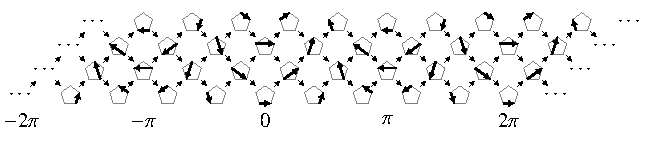
\includegraphics[width=0.96\textwidth]{figures/Fig_045_PDF107_Book095.pdf}
  % [Fig] 原书 p.95
\end{figure}

图中按网格排列对象：横轴是线段的相位，纵轴是线段起点与终点之间的逆时针角差。因此，移位算子是一个滑移反射：它使相位增加 $\pi$，并交换起点与终点；几何上等于先平移 $\pi$，再作一次水平反射。

也可以为线性箭图表示的导出范畴画出同一幅图，并在其中清楚地辨认子范畴 $S^\bullet$、$\mathrm{mod}^\bullet Q$ 和 $P^\bullet$：
\begin{figure}[H]\centering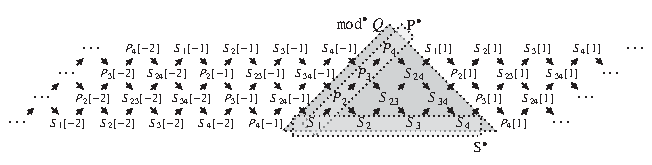
\includegraphics[width=0.96\textwidth]{figures/Fig_046_PDF108_Book096.pdf}
  % [Fig] 原书 p.96
\end{figure}

几何解释还显示，这个范畴有一个特殊的自等价 $R$：它将所有线段旋转
\[
  \frac{2\pi}{n+1}
\]
，同时给所有相位加上同一个角度。从几何角度看，这个自等价显而易见；但若从 $D\mathrm{mod}^\bullet Q$ 的角度看，它就相当深刻。该函子把一些表示映到另一些表示，例如当 $i>2$ 时，$S_i$ 映到 $S_{i-1}$；但 $S_1$ 被映到表示 $P_n[1]$ 的移位。在表示论中，这个函子也称为 Auslander–Reiten 平移\index{auslanderreitenpingyi@Auslander–Reiten 平移|hyperpage}（或按旋转方向不同称其逆函子），在图中对应沿水平方向平移 $\frac{2\pi}{n+1}$。
% [Tutor Note: 旋转 $R$ 在几何侧只是把多边形转过 $2\pi/(n+1)$，但它在表示论侧就是 Auslander--Reiten 平移 $\tau$：这是导出范畴的固有自等价，一般不能由 $\mathrm{mod}\,Q$ 的普通自等价实现。它把 $S_1$ 送到 $P_n[1]$ 而非某个简单模，正说明必须使用导出范畴；这也是图中 $S_1[1]$ 与 $P_n[1]$ 并列出现的原因。]

\begin{note}\phantomsection\label{note:rolled-up-linear-quiver}
\textbf{注 4.39.} 对第二种几何解释，我们只使用了 $\mathbb Z_2$-分次版本。这意味着可以忘掉线段的相位；范畴 $DS^\pm$ 是 $DS^\bullet$ 的 wrapped 版本，其中只含有 $\mathrm{mod}\,Q$ 的两个副本，并将它们粘合成一个圆柱：
\begin{figure}[H]\centering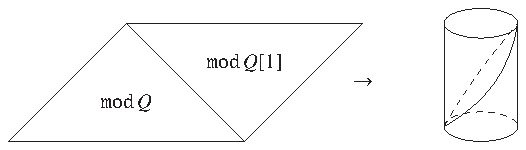
\includegraphics[width=0.78\textwidth]{figures/Fig_047_PDF108_Book096.pdf}
  % [Fig] 原书 p.96
\end{figure}
\end{note}

\subsection{克罗内克箭图}\label{subsec:picturing-kronecker-quiver}
对克罗内克箭图而言，所有相位水平的曲线都形如 $B(-,n)$。若只按相位作为横轴作图，它们都会落在同一点。为区分它们，我们把它们放进一个宽度由 $\lambda$ 参数化、高度由 $n$ 参数化的方框中。这样，在相位为 $\pi$ 的整数倍处得到一列对象。塔中每个对象都通过单射 $B(\lambda,n)\hookrightarrow B(\lambda,n+1)$ 与上方对象相连，并通过投射 $B(\lambda,n)\twoheadrightarrow B(\lambda,n-1)$ 与下方对象相连。不同 $\lambda$ 的带对象之间没有次数 $0$ 态射。

奇数大小的弦对象具有互不相同的相位：
\[
  S(0,2k+1)\text{ 的相位为 }\frac\pi2-\tan^{-1}(k),
  \qquad
  S(1,2k+1)\text{ 的相位为 }-\frac\pi2+\tan^{-1}(k+1).
\]
每个对象都通过两个次数 $0$ 态射与下一个对象相连，这两个态射分别来自左侧和右侧的嵌入。子范畴 $\mathrm{mod}^\bullet Q$ 由相位属于 $(-\frac\pi2,\frac\pi2]$ 的所有对象组成：
\begin{figure}[H]\centering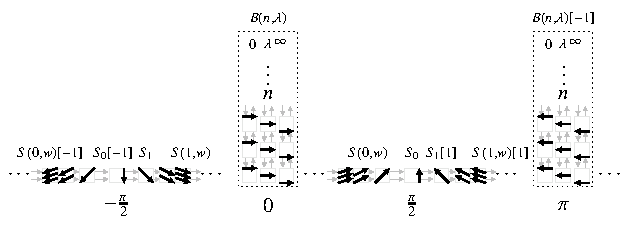
\includegraphics[width=0.96\textwidth]{figures/Fig_048_PDF109_Book097.pdf}
  % [Fig] 原书 p.97
\end{figure}

这幅图显示了范畴的一种对称性：把所有奇数长度的弦对象向右平移 $1$。在圆柱上，这对应于一个 Dehn 扭转：让上边界圆向左转一整圈，就像拧开罐子的盖子。每条穿过圆柱的曲线都因此多出一圈扭转：$S(1,w)$ 变为 $S(1,w+2)$，$S(0,w)$ 变为 $S(0,w-2)$，而 $S_0$ 变为 $S_1[1]$。同样，从曲线角度看这个等价很自然，但从箭图角度看则很不寻常。

第二种对称性来自 $\mathbb P^1$ 上层的几何解释。从这一角度看，每个 $g\in\mathrm{PGL}_2(\mathbb C)$ 都诱导射影直线上的变换，将层 $S(p,n)$ 变为 $S(g\cdot p,n)$。局部自由层在这些变换下不变。这个对称性从 $\mathbb P^1$ 的角度显而易见；但从带标记点的圆柱角度看就很不自然，因为它会混合弦对象与带对象。

\subsection{循环箭图}\label{subsec:picturing-cyclic-quiver}
在这幅图中，除移位外只有两个相位。在 $\frac\pi2$ 处是所有投射模，它们通过箭头 $a_i$ 循环相连；在 $0$ 处是所有有限维模，我们按维数将它们沿竖直方向排列。弦模 $S(i,w)$ 可按起点循环排列。这样便得到一个管状图：每一层高度上，模都通过菱形网格与相邻两层相连。在高度为 $n$ 的倍数处，还会出现一层带对象：
\begin{figure}[H]\centering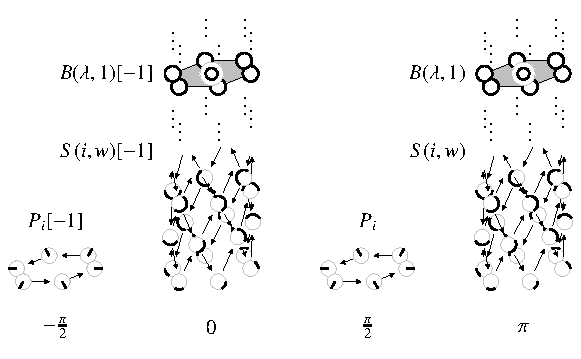
\includegraphics[width=0.94\textwidth]{figures/Fig_049_PDF110_Book098.pdf}
  % [Fig] 原书 p.98
\end{figure}

这里也有对称性。第一种对称性把 $S(i,w)$ 映到 $S(i+1,w)$，把 $P_i$ 映到 $P_{i+1}$，但固定所有 $B(\lambda,k)$。它对应于把带标记点的圆柱旋转 $\frac{2\pi}{n}$。第二种对称性固定所有 $S(i,w)$ 和 $P_i$，但把 $B(\lambda,k)$ 缩放为 $B(r\lambda,k)$；这对应于把轨形 $[\mathbb A^1/G]$ 按比例因子 $r$ 缩放。

\section{同调镜像对称初探}\label{sec:first-glimpse-hms}
\takeaway{箭图表示、$A$ 模型（曲面上曲线的交理论，即 Fukaya 范畴的雏形）与 $B$ 模型（相干层、矩阵分解、奇点范畴）给出同一批 $A_\infty$ 范畴的不同实现；它们本身不必等价，但取导出范畴后等价——这就是同调镜像对称的第一批实例。}
本章中，我们看到某些箭图的表示论可以用两种不同的几何方式来解释。
\begin{itemize}
  \item 第一种解释涉及曲面上曲线的交理论，由此得到一个 $A_\infty$ 范畴：对象是嵌入曲线，态射是交点处（角）的线性组合。这些范畴是更大一类范畴的初步例子，这一类范畴称为 Fukaya 范畴。

  一般来说，Fukaya 范畴描述的是 $2n$ 维辛流形中某些 $n$ 维子流形（称为拉格朗日子流形）的交理论。与曲面上的曲线类似，两个拉格朗日子流形通常会在若干点相交，因此可用交点作为态射空间的一组基。这样的范畴有许多不同版本：Fukaya 范畴、wrapped Fukaya 范畴、Fukaya–Seidel 范畴等。这类构造常称为 A 模型，因为它们与物理学中的 IIA 型超弦理论有关。

  \item 第二种解释涉及复代数簇上的相干层。相干层是向量丛的推广，而态射则度量层之间的映射（次数 $0$）、映射存在的障碍和层之间的扩张（高次）。这类范畴也有许多版本：相干层的导出范畴、矩阵分解范畴、奇点范畴等。这些构造称为 B 模型，因为它们出现在 IIB 型弦理论中。
\end{itemize}

不同模型（箭图、A 模型和 B 模型）给出的 $A_\infty$ 范畴并非完全等价，但取导出范畴后就会等价。这个过程为范畴添加了更多对象，使其在某种意义下更为良好，同时不改变其表示论。

下面列出目前已经建立对应关系的模型。列表看起来不长，但它只是冰山一角。事实上，只要有一些创造性，几乎可以为任何 A 模型找到合适的 B 模型，反之亦然。这一现象由超弦理论预言，如今称为同调镜像对称。下一部分将详细考察这一思想。
\begin{figure}[H]\centering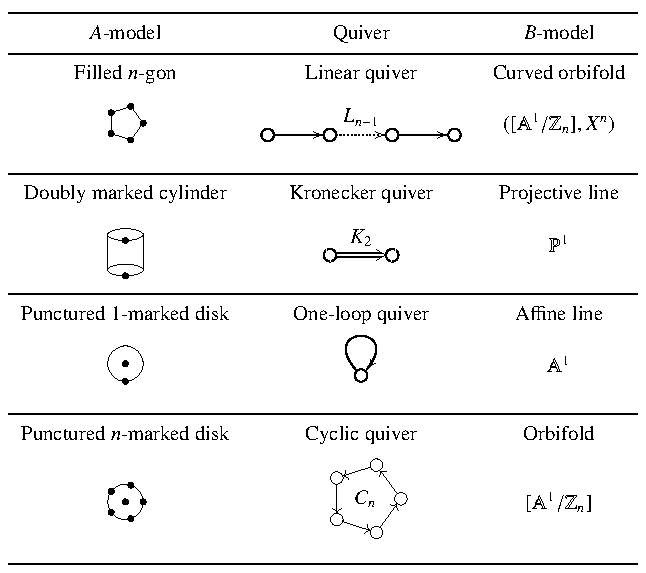
\includegraphics[width=0.92\textwidth]{figures/Fig_050_PDF111_Book099.pdf}
  % [Fig] 原书 p.99
\end{figure}

\section{练习}\label{sec:chapter4-exercises}
\begin{exercise}\label{exer:quiver-orientation-independence}
设 $Q$ 是一个有 $n$ 个顶点、$n-1$ 条箭头的箭图，顶点沿直线排列，但箭头方向不必一致。证明：在等价意义下，$D\mathrm{mod}^\bullet\mathbb C Q$ 不依赖于箭头的定向。（提示：在 $(n+1)$ 边形中选取一些直线，使它们的自同态环为 $\mathbb C Q$。）
\end{exercise}

\begin{exercise}\label{exer:linear-quiver-generators}
设 $Q$ 是有 $n$ 个顶点的线性箭图，且 $X_1,\ldots,X_k\in D\mathrm{mod}^\bullet Q$ 是分别对应于 $(n+1)$ 边形中分次线段 $L_1,\ldots,L_k$ 的对象。证明：$X_1,\ldots,X_k$ 分裂生成 $D\mathrm{mod}^\bullet Q$，当且仅当这些线段的端点覆盖多边形的所有顶点。
\end{exercise}

\begin{exercise}\label{exer:full-strong-exceptional-sequences}
导出范畴 $D\mathcal C^\bullet$ 中的满强例外序列，是一个有序对象列 $X_1,\ldots,X_k$，满足它分裂生成该范畴，并且
\[
  D\mathcal C^d(X_i,X_j)=
  \begin{cases}
    0,&d\ne0\text{ 或 }i>j,\\
    \mathbb C,&i=j,\ d=0.
  \end{cases}
\]
换言之，所有非平凡态射都在次数 $0$，并且只可能从序列中较早的对象指向较后的对象。确定有三个顶点的线性箭图 $Q$ 所对应的 $D\mathrm{mod}^\bullet Q$ 中所有满强例外序列。
\end{exercise}

\begin{exercise}\label{exer:linear-quiver-autoequivalences}
确定有 $n$ 个顶点的线性箭图 $Q$ 所对应的 $D\mathrm{mod}^\bullet Q$ 的自等价群。
\end{exercise}

\begin{exercise}\label{exer:two-one-cylinder-quiver}
考虑一条边界圆上有两个标记点、另一条边界圆上有一个标记点的圆柱。试把该曲面上线段的交理论解释为下图所示箭图的导出范畴，并描述该范畴中的所有不可分解对象。
\begin{figure}[H]\centering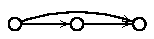
\includegraphics[width=0.48\textwidth]{figures/Fig_051_PDF112_Book100.pdf}
  % [Fig] 原书 p.100
\end{figure}
\end{exercise}

\begin{exercise}\label{exer:spherical-objects-projective-line}
若对象 $X\in D\mathcal C^\bullet$ 的自同态环是 $n$ 维球面的上同调环
\[
  D\mathcal C^\bullet(X,X)\cong\mathbb C\oplus\mathbb C[n],
\]
则称 $X$ 为 $n$-球对象。确定 $D\mathrm{Coh}^\bullet\mathbb P^1$ 中所有 $1$-球对象。
\end{exercise}

\begin{exercise}\label{exer:orbifold-disjoint-disks}
设 $G=\langle g\mid g^{kl}=1\rangle$，并令 $G$ 作用于 $\mathbb C[X]$，满足
\[
  gX=e^{2\pi i/k}X.
\]
证明：$D\mathrm{Coh}^\bullet[\mathbb A^1/G]$ 可用 $l$ 个互不相交、各有一个穿孔且边界上各有 $k$ 个标记点的圆盘的交理论来描述。
\end{exercise}

\begin{exercise}\label{exer:two-punctured-sphere-hms}
证明：有两个穿孔的球面的 A 模型可由 $D\mathbb C[X,X^{-1}]$ 描述，而相应的 B 模型是
\[
  \mathbb A^1\setminus\{0\}=\mathbb P^1\setminus\{0,\infty\}.
\]
因此，A 模型和 B 模型具有相同的底层拓扑空间。
\end{exercise}

\begin{exercise}\label{exer:punctured-orbifold-laurent}
令 $G=\langle g\mid g^n=1\rangle$ 作用于 $\mathbb C[X,X^{-1}]$，满足
\[
  gX=e^{2\pi i/n}X.
\]
证明：$[\mathbb A^1\setminus\{0\}/G]$ 与 $\mathbb A^1\setminus\{0\}$ 的 $B$ 模型等价。
\end{exercise}

\begin{exercise}\label{exer:orbifold-di[已脱敏]}
证明：范畴 $\operatorname{MF}^{\pm}(\mathbb C[X],X^n)$ 可以解释为一个圆盘的 $A$ 模型，其中边界上有一个标记点，圆盘中心有一个 $n$ 阶轨形点。为理解这一点，考虑 $n$ 重覆盖
\[
  \pi\colon D\to D,\qquad z\longmapsto z^n.
\]
$A$ 模型中的对象是覆盖下方的曲线，而乘积则由覆盖空间上方的多边形给出。
\end{exercise}

\chapterreview{%
\textbf{全章地位。}本章是全书第一部完整的词典：同一批不可分解对象，既能写成箭图的表示，又能画成曲面上的曲线，还能读成层。作者用三个可以完全分类的例子把 A 模型与 B 模型并置，同调镜像对称于是在最低维上成为可逐条验证的定理，而不只是物理猜想。

\textbf{知识脉络。}从路径代数 $\mathbb C Q$ 出发，先由基本投射模与基本简单模得到包含关系 $DS^\bullet\subset D\mathrm{mod}^\bullet Q\subset DP^\bullet$；无有向圈时三者等价，有圈时三者分离，这就迫使读者进入导出范畴。随后把三个箭图逐个画出来：线性箭图给出 $(n+1)$ 边形中的分次线段，克罗内克箭图给出圆柱上的弦与带，循环箭图给出带无穷远端的圆柱。再把角读成态射、把锥读成拼接、把多边形读成高阶乘积，交理论模型便与 $A_\infty$ 结构合为一体。最后一节换到代数几何一侧，用 $\mathbb A^1$、$\mathbb P^1$、轨形 $[\mathbb A^1/\mathbb Z_n]$ 上的相干层和 Landau--Ginzburg 模型的奇点范畴重讲同一批例子，两种解释在导出范畴层面重合。

\textbf{核心结论。}（1）$DS^\bullet\subset D\mathrm{mod}^\bullet Q\subset DP^\bullet$，且当 $Q$ 无有向圈时三者都是等价；有圈时 $DS^\bullet$ 只含幂零模，$D\mathrm{mod}^\bullet Q$ 则遗漏顶点位于有向圈上的基本投射模 $P_v$。（2）不可分解对象分类：线性箭图为 $S_{ij}$ 的移位；克罗内克箭图为弦对象 $S(i,w)$ 与带对象 $B(\lambda,n)$，偶长弦对象是 $\lambda\to0,\infty$ 时带对象的极限；循环箭图的 $S(i,w)$、$B(k,\lambda)$、$P_i$ 分别落在 $DS^\bullet$、$D\mathrm{mod}^\bullet Q$、$DP^\bullet$ 中。（3）态射由交点处的角生成，次数为 $(\beta-(\theta_2-\theta_1))/\pi$；锥对应沿角拼接线段，多边形则给出 $\mu(\alpha_1,\ldots,\alpha_{k-1})=\pm\overline\alpha_k$。（4）几何实现：线性箭图的交理论模型给出 $DS^\bullet\cong_\infty\mathrm{Polygon}_{n+1}^\bullet$；克罗内克箭图在导出层面等价于 $\mathbb P^1$ 上的相干层；循环箭图对应轨形相干层，其 Landau--Ginzburg 奇点范畴又给出线性箭图 $L_{n-1}$。

\textbf{辨析与提醒。}其一，三个范畴的记号必须随时区分：同一箭图表示在 $DS^\bullet$ 中表现为 $S_\rho$，在 $D\mathrm{mod}^\bullet Q$ 中表现为模 $M_\rho$，在 $DP^\bullet$ 中表现为扭曲复形 $P_\rho$，三者只在幂零情形才重合。其二，相位与定向是全章最容易出错处：反向线段相位加 $\pi$，移位加 $\pi$，角的次数公式中 $\beta$ 与 $\theta_i$ 必须同向取；只给其中一个量加 $\pi$ 会整体差一次移位。其三，循环箭图 $C_n$ 对应的不是 $L_n$ 而是 $L_{n-1}$，奇点范畴一节的这个下标差一是结构使然，不是笔误。

\textbf{评注。}作者把“导出范畴才是正确栖居地”这一信念放在最前面，而不是先讲高维辛几何，这是全书最有效的教学决定：读者先在能画全的例子里看到等价真正发生，之后遇到泡、Novikov 环与虚拟基本类时，才知道那些技术是为谁服务的。代价同样明显——一切都在曲线上进行，高维才有的现象被完全抹平，读者容易把“箭图就是 Fukaya 范畴”当成一般事实。另一处值得称道的是把弦对象与带对象的极限关系讲透（$B(\lambda,n)$ 在参数边界退化为偶长弦对象），这实际上是后文 partially wrapped 与局部化思想的胚胎。阅读时建议亲手算一遍三种箭图的态射表，再把范畴图景中的旋转看成 Auslander--Reiten 平移，收获会比读定义大得多。}
